\chapter{Algoritmi}\label{algoritmi}

In questo capitolo vengono presentati alcuni degli algoritmi più utilizzati in letteratura per feedback impliciti ed espliciti.

\section{Notazione}\label{notazione}

La notazione utilizzata è la seguente:

\begin{itemize}
    \item \textit{user}: l'utente/i
    \item \textit{item}: l'elemento/i
    \item \textit{rating}: valutazione/i
    \item $m$: numero di \textit{user}
    \item $n$: numero di \textit{item}
    \item $R$: matrice che contiene l'insieme di tutti i \textit{rating}/interazioni (per i feedback impliciti)
    \item $R_{train}$, $R_{test}$ e $\hat{R}$ indicano il \textit{training set}, il \textit{test set} e l'insieme dei \textit{rating} previsti
    \item $U$ : l'insieme di tutti gli \textit{user} $u$ e $v$ indicano gli \textit{user}
    \item $I$ : l'insieme di tutti gli \textit{item} $i$ e $j$ indicano gli \textit{item}
    \item $U_i$ : l'insieme di tutti gli \textit{user} che hanno valutato l'\textit{item} $i$
    \item $U_{ij}$ : l'insieme di tutti gli \textit{user} che hanno valutato sia l'\textit{item} $i$ che l'\textit{item} $j$
    \item $I_u$ : l'insieme di tutti gli \textit{item} valutati dallo \textit{user} $u$
    \item $I_{uv}$ : l'insieme di tutti gli \textit{item} valutati sia dallo \textit{user} $u$ che dallo \textit{user} $v$
    \item $r_{ui}$ : il \textit{rating} \textit{vero} dello \textit{user} $u$ per l'\textit{item} $i$
    \item $\hat{r}_{ui}$ : il \textit{rating} \textit{stimato} dello \textit{user} $u$ per l'\textit{item} $i$
    \item $b_u$: \textit{bias} dello \textit{user} $u$, misura quanto in media lo \textit{user} tende a dare valutazioni più alte o più basse rispetto alla media generale. Se tende sempre a dare voti più alti della media $b_u$ sarà positivo; se tende a dare voti più bassi, sarà negativo
    \item $b_u$: \textit{bias} dell'\textit{item} $i$, misura quanto un \textit{item} tende a ricevere valutazioni più alte o più basse rispetto alla media, indipendentemente dallo \textit{user}. Per esempio, un \textit{item} molto popolare potrebbe avere un $b_u$ positivo perché riceve in media voti più alti rispetto alla media generale
    \item $b_{ui}$ : il \textit{rating} di base dello \textit{user} $u$ per l'\textit{item} $i$, viene definito \textit{baseline estimate}: $b_{ui} = \mu + b_u + b_i$
    \item $\mu$ : la media di tutti i \textit{rating}
    \item $\mu_u$ : la media di tutti i \textit{rating} dati dallo \textit{user} $u$
    \item $\mu_i$ : la media di tutti i \textit{rating} date all'\textit{item} $i$
    \item $\sigma_u$ : la deviazione standard di tutti i \textit{rating} dati dallo \textit{user} $u$
    \item $\sigma_i$ : la deviazione standard di tutte le valutazioni date all'\textit{item} $i$
    \item $N_i^k(u)$ : i $k$ vicini più prossimi dello \textit{user} $u$ che hanno valutato l'\textit{item} $i$. Questo insieme è calcolato utilizzando una metrica di similarità
    \item $N_u^k(i)$ : i $k$ vicini più prossimi dell'\textit{item} $i$ che sono valutati dallo \textit{user} $u$. Questo insieme è calcolato utilizzando una metrica di similarità
    \item $\gamma$: iperparametro, il \textit{learning rate} utilizzato per l'algoritmo \textit{Stocastic Gradient Descent}
    \item $\lambda$: iperparametro, corrisponde al fattore di regolarizzazione nella funzione obbiettivo
    \item $\hat{y}_{uij}$: \textit{score} che rappresenta la preferenza dello \textit{user} \textit{i} per l'\textit{item} \textit{i} rispetto all'\textit{item} \textit{j}
    \item $N$: numero di epoche per l'algoritmo \textit{Stocastic Gradient Descent}
    \item $k$: dimensione dello spazio latente negli algoritmi di \textit{Matrix Factorization} o il numero dei \textit{neighbors} negli algoritmi della famiglia \textit{KNN}
\end{itemize}


\section{Tassonomia degli algoritmi}

Viene presentata una tassonomia degli algoritmi di \textit{recommendation}.

\begin{itemize}[label=\textbullet]

    \item \textit{AutoRec}
    \begin{itemize}
        \item feedback: implicito ed esplicito
        \item tecnica: \textit{Autoencoder}
        \item approccio: \textit{Model-based}
        \item filtering: \textit{Collaborative Filtering}
    \end{itemize}

    \item \textit{NCF (Neural Collaborative Filtering)}
    \begin{itemize}
        \item feedback: implicito ed esplicito
        \item tecnica: \textit{Reti Neurali}
        \item approccio: \textit{Model-based}
        \item filtering: \textit{Collaborative Filtering}
    \end{itemize}

    \item \textit{DeepFM}
    \begin{itemize}
        \item feedback: implicito ed esplicito
        \item tecnica: \textit{Matrix Factorization} / \textit{Reti Neurali}
        \item approccio: \textit{Model-based}
        \item filtering: \textit{Collaborative Filtering} (potrebbe anche essere \textit{Content-based})
    \end{itemize}

    \item \textit{KNN (K-Nearest Neighbors)}
    \begin{itemize}
        \item feedback: esplicito
        \item tecnica: \textit{Memory-based} (calcola la \textit{somiglianza} tra utenti o item)
        \item approccio: \textit{Memory-based}
        \item filtering: \textit{Collaborative Filtering}
    \end{itemize}

    \item \textit{Slope One}
    \begin{itemize}
        \item feedback: esplicito
        \item tecnica: \textit{Model-based} (calcola le \textit{deviazioni medie} tra gli item)
        \item approccio: \textit{Model-based}
        \item filtering: \textit{Collaborative Filtering}
    \end{itemize}

    \item \textit{SVD (Singular Value Decomposition)}
    \begin{itemize}
        \item feedback: esplicito
        \item tecnica: \textit{Matrix Factorization}
        \item approccio: \textit{Model-based}
        \item filtering: \textit{Collaborative Filtering}
    \end{itemize}

    \item \textit{SVD++}
    \begin{itemize}
        \item feedback: implicito ed esplicito
        \item tecnica: \textit{Matrix Factorization} (un'estensione di \textit{SVD})
        \item approccio: \textit{Model-based}
        \item filtering: \textit{Collaborative Filtering}
    \end{itemize}

    \item \textit{NMF (Non-Negative Matrix Factorization)}
    \begin{itemize}
        \item feedback: esplicito
        \item tecnica: \textit{Matrix Factorization} (con vincoli di \textit{non negatività})
        \item approccio: \textit{Model-based}
        \item filtering: \textit{Collaborative Filtering}
    \end{itemize}

    \item \textit{CoClustering}
    \begin{itemize}
        \item feedback: esplicito
        \item tecnica: \textit{Clustering} (raggruppa simultaneamente \textit{utenti} e \textit{item})
        \item approccio: \textit{Model-based}
        \item filtering: \textit{Collaborative Filtering}
    \end{itemize}

    \item \textit{ALS (Alternating Least Squares)}
    \begin{itemize}
        \item feedback: implicito ed esplicito
        \item tecnica: \textit{Matrix Factorization}
        \item approccio: \textit{Model-based}
        \item filtering: \textit{Collaborative Filtering}
    \end{itemize}

    \item \textit{BPR (Bayesian Personalized Ranking)}
    \begin{itemize}
        \item feedback: implicito
        \item tecnica: \textit{Matrix Factorization} (ottimizzato per problemi di \textit{ranking})
        \item approccio: \textit{Model-based}
        \item filtering: \textit{Collaborative Filtering}
    \end{itemize}

    \item \textit{LMF (Logistic Matrix Factorization)}
    \begin{itemize}
        \item feedback: implicito
        \item tecnica: \textit{Matrix Factorization} (usa un \textit{modello logistico})
        \item approccio: \textit{Model-based}
        \item filtering: \textit{Collaborative Filtering}
    \end{itemize}

    \item \textit{LightFM}
    \begin{itemize}
        \item feedback: impliciti ed espliciti
        \item tecnica: \textit{Hybrid} (combina \textit{Matrix Factorization} e \textit{Content-based Features})
        \item approccio: \textit{Model-based}
        \item filtering: \textit{Hybrid} (\textit{Collaborative Filtering} e \textit{Content-based Filtering})
    \end{itemize}

\end{itemize}

\section{Algoritmi per il feedback esplicito}\label{algoritmi-per-feedback-esplicito}

\subsection{KNN (K-Nearest Neighbors)}\label{knn}
Si tratta di algoritmi derivati direttamente da un approccio di base basato sui \textit{Nearest Neighbors}.

Gli algoritmi ispirati al KNN (\textit{K Nearest Neighbors}) sono una classe di algoritmi di \textit{recommendation} che si basano sull'idea che gli \textit{user} simili tendono a valutare gli stessi \textit{item} in modo simile. Questi algoritmi sono semplici da implementare e possono essere molto efficaci per problemi a piccola scala.

Il numero effettivo di vicini che vengono considerati per calcolare la predizione è minore o uguale a $k$: potrebbero non esserci abbastanza vicini e/o gli insiemi $N_i^k(u)$ e $N_u^k(i)$ includono solo vicini per i quali la misura di similarità è positiva (non avrebbe senso considerare \textit{user} o \textit{item} correlati negativamente).

$k$ è un iperparametro di ciascun algoritmo.

Alcune misure di similarità, sia per \textit{user} che per \textit{item}, sono:
\begin{itemize}
    \item Coseno:
        \[
        \text{cosine sim}(u, v) = \frac{\sum\limits_{i \in I_{uv}} r_{ui} \cdot r_{vi}}{\sqrt{\sum\limits_{i \in I_{uv}} r_{ui}^2} \cdot \sqrt{\sum\limits_{i \in I_{uv}} r_{vi}^2}}
        \]
        oppure, per \textit{item}
        \[
        \text{cosine sim}(i, j) = \frac{\sum\limits_{u \in U_{ij}} r_{ui} \cdot r_{uj}}{\sqrt{\sum\limits_{u \in U_{ij}} r_{ui}^2} \cdot \sqrt{\sum\limits_{u \in U_{ij}} r_{uj}^2}}
        \]
    \item \textit{Mean Square Difference} (MSD):
        \[
        \text{msd}(u, v) = \frac{1}{|I_{uv}|} \cdot \sum\limits_{i \in I_{uv}} (r_{ui} - r_{vi})^2
        \]
        oppure, per \textit{item}
        \[
        \text{msd}(i, j) = \frac{1}{|U_{ij}|} \cdot \sum\limits_{u \in U_{ij}} (r_{ui} - r_{uj})^2
        \]
        La similarità è calcolata come:
        \begin{align*}
            \text{msd sim}(u, v) &= \frac{1}{\text{msd}(u, v) + 1} \\
            \text{msd sim}(i, j) &= \frac{1}{\text{msd}(i, j) + 1}
        \end{align*}
        Il termine $+1$ viene aggiunto per evitare divisioni per zero.
    \item Pearson: Il coefficiente di correlazione di Pearson può essere visto come una similarità del coseno centrato sulla media. Se non ci sono \textit{item} comuni, la similarità è 0 (non -1).
        \[
        \text{pearson sim}(u, v) = \frac{\sum\limits_{i \in I_{uv}} (r_{ui} - \mu_u) \cdot (r_{vi} - \mu_v)}{\sqrt{\sum\limits_{i \in I_{uv}} (r_{ui} - \mu_u)^2} \cdot \sqrt{\sum\limits_{i \in I_{uv}} (r_{vi} - \mu_v)^2}}
        \]
        oppure, per \textit{item}
        \[
        \text{pearson sim}(i, j) = \frac{\sum\limits_{u \in U_{ij}} (r_{ui} - \mu_i) \cdot (r_{uj} - \mu_j)}{\sqrt{\sum\limits_{u \in U_{ij}} (r_{ui} - \mu_i)^2} \cdot \sqrt{\sum\limits_{u \in U_{ij}} (r_{uj} - \mu_j)^2}}
        \]
    \item Pearson con baseline \cite{Recommendation_book}: calcola il coefficiente di correlazione di Pearson (ridotto) tra tutte le coppie di \textit{user} (o \textit{item}) utilizzando le baseline anziché le medie. Il parametro di riduzione aiuta a evitare l'overfitting quando sono disponibili solo poche valutazioni. Se non ci sono \textit{item} comuni, la similarità è 0 (non -1). Introduce un nuovo iperparametro che corrisponde alla riduzione (o \textit{``shrinkage''}). Se impostato uguale a 0, non viene applicata nessuna riduzione.
        \[
        \text{pearson baseline sim}(u, v) = \hat{\rho}_{uv} = \frac{\sum\limits_{i \in I_{uv}} (r_{ui} - b_{ui}) \cdot (r_{vi} - b_{vi})}{\sqrt{\sum\limits_{i \in I_{uv}} (r_{ui} - b_{ui})^2} \cdot \sqrt{\sum\limits_{i \in I_{uv}} (r_{vi} - b_{vi})^2}}
        \]
        oppure, per \textit{item}
        \[
        \text{pearson baseline sim}(i, j) = \hat{\rho}_{ij} = \frac{\sum\limits_{u \in U_{ij}} (r_{ui} - b_{ui}) \cdot (r_{uj} - b_{uj})}{\sqrt{\sum\limits_{u \in U_{ij}} (r_{ui} - b_{ui})^2} \cdot \sqrt{\sum\limits_{u \in U_{ij}} (r_{uj} - b_{uj})^2}}
        \]
        Il coefficiente ridotto si calcola come:
        \begin{align*}
            \text{pearson baseline shrunk sim}(u, v) &= \frac{|I_{uv}| - 1}{|I_{uv}| - 1 + \text{shrinkage}} \cdot \hat{\rho}_{uv} \\
            \text{pearson baseline shrunk sim}(i, j) &= \frac{|U_{ij}| - 1}{|U_{ij}| - 1 + \text{shrinkage}} \cdot \hat{\rho}_{ij}
        \end{align*}
        Per il calcolo della baseline, si consideri la parte di \ref{knn_baseline}.
\end{itemize}

Altro iperparametro da considerare è il supporto minimo, che corrisponde al numero minimo di \textit{item} in comune o il numero minimo di \textit{user} in comune affinché la similarità non sia zero, i.e., se $|I_{uv}| < \text{min support}$, allora $\text{sim}(u, v) = 0$. Lo stesso vale per gli \textit{item}.

\subsubsection{KNN base}

L'algoritmo KNN base è l'algoritmo più semplice. Prevede il  \textit{rating} di un \textit{user} $u$ per un \textit{item} $i$ come la media ponderata dei \textit{rating} degli $k$ vicini più simili di $u$ o $i$, a seconda che si utilizzi un approccio basato sugli \textit{user} o sugli \textit{item}.

La predizione viene calcolata come:

\[
\hat{r}_{ui} = \frac{\sum\limits_{v \in N^k_i(u)} \text{sim}(u, v) \cdot r_{vi}}{\sum\limits_{v \in N^k_i(u)} \text{sim}(u, v)}
\]

oppure, per \textit{item}

\[
\hat{r}_{ui} = \frac{\sum\limits_{j \in N^k_u(i)} \text{sim}(i, j) \cdot r_{uj}}{\sum\limits_{j \in N^k_u(i)} \text{sim}(i, j)}
\]

dipendentemente dall'approccio utilizzato.

\subsubsection{KNN con la media}

L'algoritmo è una variante dell'algoritmo \textit{KNN} base che tiene conto della media dei \textit{rating} degli \textit{user} o degli \textit{item}.

La predizione viene calcolata come:

\[
\hat{r}_{ui} = \mu_u + \frac{\sum\limits_{v \in N_k(u)} \text{sim}(u, v) \cdot (r_{vi} - \mu_v)}{\sum\limits_{v \in N_k(u)} \text{sim}(u, v)}
\]

oppure, per \textit{item}

\[
\hat{r}_{ui} = \mu_i + \frac{\sum\limits_{j \in N^k_u(i)} \text{sim}(i, j) \cdot (r_{uj} - \mu_j)}{\sum\limits_{j \in N^k_u(i)} \text{sim}(i, j)}
\]

dipendentemente dall'approccio utilizzato.

\subsubsection{KNN normalizzato}

L'algoritmo è una variante dell'algoritmo che utilizza la media con l'aggiunta della normalizzazione \textit{z-score}, con la deviazione standard dello \textit{user} o dell'\textit{item}, dei \textit{rating} corrispondenti prima di calcolare la similarità.

La predizione viene calcolata come:

\[
\hat{r}_{ui} = \mu_u + \sigma_u \frac{\sum\limits_{v \in N^k_i(u)} \text{sim}(u, v) \cdot (r_{vi} - \mu_v) / \sigma_v}{\sum\limits_{v \in N^k_i(u)} \text{sim}(u, v)}
\]

oppure, per \textit{item}

\[
\hat{r}_{ui} = \mu_i + \sigma_i \frac{\sum\limits_{j \in N^k_u(i)} \text{sim}(i, j) \cdot (r_{uj} - \mu_j) / \sigma_j}{\sum\limits_{j \in N^k_u(i)} \text{sim}(i, j)}
\]

dipendentemente dall'approccio utilizzato.

\subsubsection{KNN con baseline}\label{knn_baseline}

L'algoritmo KNN con baseline~\cite{KNN_baseline} è una variante dell'algoritmo base che tiene conto degli effetti dei bias degli \textit{user} o degli \textit{item}.

La predizione viene calcolata come:

\[
\hat{r}_{ui} = b_{ui} + \frac{\sum\limits_{v \in N^k_i(u)} \text{sim}(u, v) \cdot (r_{vi} - b_{vi})}{\sum\limits_{v \in N^k_i(u)} \text{sim}(u, v)}
\]

oppure, per \textit{item}

\[
\hat{r}_{ui} = b_{ui} + \frac{\sum\limits_{j \in N^k_u(i)} \text{sim}(i, j) \cdot (r_{uj} - b_{uj})}{\sum\limits_{j \in N^k_u(i)} \text{sim}(i, j)}
\]

dipendentemente dall'approccio utilizzato.

La baseline $b_{ui}$ viene calcolata come:

\[
b_{ui} = \mu + b_u + b_i
\]

Per calcolare $b_u$ e $b_i$, occorre minimizzare il seguente errore quadratico regolarizzato:

\[
\sum\limits_{r_{ui} \in R_{train}} \left(r_{ui} - \mu + b_u + b_i\right)^2 + \lambda \left(b_u^2 + b_i^2 \right).
\]

Il termine di regolarizzazione $\lambda \left(b_u^2 + b_i^2 \right)$ serve per evitare l'overfitting penalizzando la grandezza dei parametri.

La minimizzazione può essere effettuata tramite \textit{Stochastic Gradient Descent} o \textit{Alternating Least Squares}.

Per \textit{Alternating Least Squares}, i due valori di $b_u$ e $b_i$ si ottengono come:

\[
b_i = \frac{\sum\limits_{r_{ui} \in R_{train}} (r_{ui} - \mu)}{\lambda_2 + |U_i|}
\]

e

\[
b_u = \frac{\sum\limits_{r_{ui} \in R_{train}} (r_{ui} - \mu - b_i)}{\lambda_3 + |I_u|}
\]

I punti di forza della famiglia di algoritmi \textit{KNN} sono:
\begin{itemize}
    \item semplicità: Gli algoritmi \textit{KNN} sono facili da capire e implementare. L'idea di base di trovare ``vicini" simili è intuitiva e facilmente comprensibile
    \item nessuna assunzione sui dati: l'algoritmo non fa assunzioni sulla distribuzione dei dati. Questo lo rende flessibile e adatto a una varietà di dataset
    \item aggiornamento: l'aggiunta di nuovi dati non richiede una fase di addestramento esplicita. Questo lo rende utile in ambienti in cui i dati cambiano frequentemente o per previsioni online
    \item flessibilità: \textit{KNN} può essere utilizzato sia per problemi di \textit{recommendation} basati su \textit{user} che basati su \textit{item}
\end{itemize}

Gli algoritmi soffrono anche di diverse problematiche:
\begin{itemize}
    \item costo computazionale: \textit{KNN} può essere computazionalmente costoso, soprattutto con set di dati di grandi dimensioni
    \item requisiti di memoria: \textit{KNN} richiede la memorizzazione dell'intero set di dati, il che può essere problematico per set di dati molto grandi
    \item sensibilità alla scelta di $k$: La scelta del valore di $k$ può avere un impatto significativo sulle prestazioni di \textit{KNN}. Un valore di $k$ troppo piccolo può portare a un overfitting, mentre un valore di $k$ troppo grande può portare a un underfitting. Inoltre, la ricerca dei $k$ vicini più prossimi richiede il calcolo delle distanze tra tutti i punti dati
    \item gestione della sparsità dei dati: la sparsità può rendere difficile trovare vicini significativi e quindi portare a raccomandazioni di bassa qualità
\end{itemize}

\subsection{Slope One}\label{slopeone}

L'algoritmo \textit{Slope One}, introdotto da Daniel Lemire e Anna Maclachlan~\cite{SlopeOne}, è una delle soluzioni più semplici ed efficienti di \textit{collaborative filtering}.

Le caratteristiche che lo rendono un ottimo algoritmo per la \textit{recommendation} sono:
\begin{itemize}
    \item la semplicità e facilità di implementazione
    \item velocità di calcolo: come verrà presentato più avanti alcuni valori calcolati possono essere salvati e aggiornati all'occorrenza rendendo il calcolo molto più veloce
    \item scalabilità: l'algoritmo può essere abbastanza efficace su dataset di dimensioni moderate, soprattutto se si utilizzano tecniche di compressione dei dati
    \item facilità di interpretazione
\end{itemize}

Viene proposto un predittore basato su differenze di \textit{rating} lineari che ha un costo computazionale $\mathcal{O}(nm)$ per predizione e $\mathcal{O}(mn^2)$ per addestramento.

L'algoritmo si basa sulla differenza media tra le valutazioni di due \textit{item} per predire il \textit{rating} mancante. La differenza media dei \textit{rating} di due \textit{item} $i$ e $j$ viene calcolata come:

\[
    \text{dev}(i, j) = \frac{1}{|U_{i,j}|} \sum\limits_{u \in U_{i,j}} (r_{u,i} - r_{u,j})
\]

La matrice simmetrica, definita da $\text{dev}(i, j)$, può essere computata una volta e aggiornata velocemente quando vengono aggiunti nuovi dati.

La predizione viene dunque calcolata come:

\[
    \hat{r}_{ui} = \mu_u + \frac{1}{|R_i(u)|} \sum\limits_{j \in R_i(u)} \text{dev}(i, j)
\]

dove:

\begin{itemize}
    \item $R_j = \{ i \mid i \in S(u), i \neq j, |S_{j,i}(\chi)| > 0 \}$ è l'insieme degli \textit{item} rilevanti
    \item $S(u)$ è il sottoinsieme degli \textit{item} valutati dallo \textit{user} $u$
    \item $S_{j,i}(\chi)$ è l'insieme di tutte le valutazioni $u$ nel dataset $\chi$ che contengono gli \textit{item} $i$ e $j$
\end{itemize}

\begin{figure}[H]
    \centering
    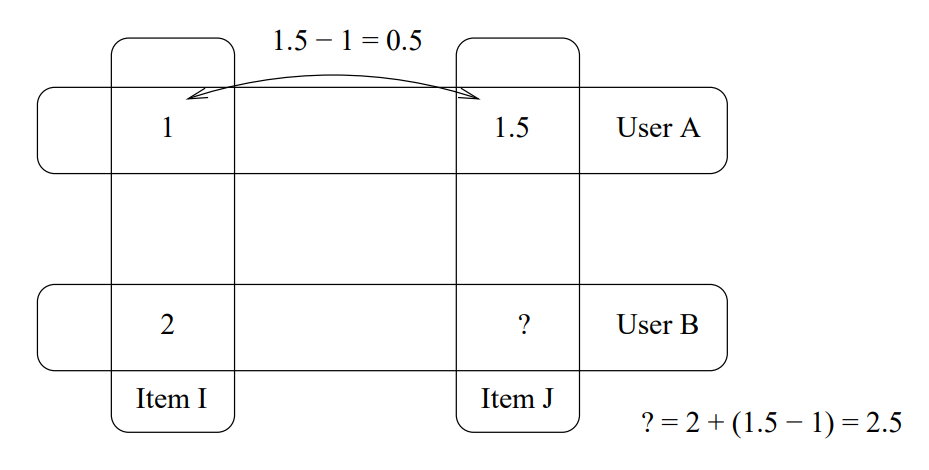
\includegraphics[keepaspectratio]{figures/algorithms/slope_one.PNG}
    \caption{Base dello schema Slope One: le valutazioni dello \textit{user} A di due \textit{item} e la valutazione  dello \textit{user} B di un \textit{item} comune vengono utilizzate per prevedere la valutazione sconosciuta dello \textit{user}.}
    \label{fig:slopeone}
\end{figure}

L'algoritmo soffre anche di diverse problematiche:
\begin{itemize}
    \item sparsità dei dati: le formule presentate prima sono approssimate considerando un dataset non sparso. Nel caso di matrici molto sparse l'algoritmo non sarà in grado di fare previsioni accurate
    \item scalabilità limitata su dataset molto grandi: la memoria necessaria per memorizzare le differenze medie dei \textit{rating} può aumentare rapidamente
    \item non tiene conto nè di personalizzazioni per \textit{user} nè di \textit{item}
    \item difficoltà a gestire grandi variazioni nelle valutazioni degli utenti
\end{itemize}

L'approccio può essere esteso a modelli ponderati e versioni più avanzate, come per esempio \textit{Weighted Slope One}, che pesa le differenze di \textit{rating} in base alla frequenza di coppie di \textit{item} valutati, e \textit{Regression-based Slope One}, che introduce funzioni non lineari per migliorare la precisione delle previsioni.

\subsection{SVD (Singular Value Decomposition)}\label{svd}

L'algoritmo SVD (\textit{Singular Value Decomposition}), è stato reso popolare da Simon Funk durante la competizione \textit{the Netflix Prize} dimostrando come modelli di fattorizzazione matriciale sono superiori alle tecniche classiche basate su \textit{nearest neighbor}\ref{knn} per
la produzione di raccomandazioni.

I modelli di \textit{Matrix Factorization} mappano gli \textit{user} e gli \textit{item} in uno spazio latente comune di dimensione $k$, che rappresenta il numero di caratteristiche latenti. Ogni \textit{item} $i$ è associato a un vettore $q_i$ di dimensione $k$, che misura quanto l'\textit{item} possieda ciascuna di queste caratteristiche latenti. Per ogni \textit{user} $u$, invece, il vettore $p_u$ misura l'interesse dello \textit{user} per gli \textit{item}. Il numero di fattori è un iperparametro dell'algoritmo.

In questo spazio, le interazioni tra \textit{user} e \textit{item} vengono modellate come prodotti scalari tra i rispettivi vettori. Lo spazio latente cerca di spiegare i \textit{rating} caratterizzando sia gli \textit{item} che gli \textit{user} in base a fattori che vengono automaticamente dedotti. Ad esempio, se gli \textit{item} sono film, i fattori potrebbero rappresentare il genere piuttosto che un altro (e.g. Azione piuttosto che Drama), profondità della trama o il concetto di ``adatto ai bambini".

Il prodotto scalare risultante cattura l'interazione tra lo \textit{user} $u$ e l'\textit{item} $i$, che corrisponde all'interesse complessivo dello \textit{user} per le caratteristiche dell'\textit{item}. Il \textit{rating} finale viene ottenuto aggiungendo anche i predittori di base, che dipendono solo dallo \textit{user} o dall'\textit{item}. Pertanto, un \textit{rating} viene predetto dalla regola~\cite{SVD_analysis}~\cite{Recommendation_book}:

\[
\hat{r}_{ui} = \mu + b_u + b_i + q_i^T p_u
\]

Dove:
\begin{itemize}
    \item $ b_u $ e $ b_i $ sono i bias dello \textit{user} $u$ e dell'\textit{item} $i$ rispettivamente. Sono una sorta di correzione basata sull'effetto dello \textit{user} e dell'\textit{item}.
    \item $ q_i^T p_u $ è il prodotto interno tra i vettori latenti dello \textit{user} e dell'\textit{item}.
\end{itemize}

Se lo \textit{user} $u$ è sconosciuto, allora il bias $b_u$ e i fattori $p_u$ vengono considerati uguali a zero. Lo stesso vale per
l'\textit{item} $i$, con $b_i$ e $q_i$ anch'essi assunti uguali a zero.

Per apprendere i parametri del modello ($b_u$, $b_i$, $p_u$, $q_i$), si minimizza l'errore quadratico regolarizzato tra i \textit{rating} reali e quelle previste. L'errore quadratico è dato da:

\[
\min \sum\limits_{(u,i) \in K} \left( (r_{ui} - \hat{r}_{ui})^2 + \lambda (\|q_i\|^2 + \|p_u\|^2 + b_u^2 + b_i^2) \right)
\]


Dove il primo termine è l'errore quadratico tra i \textit{rating} previste e reali e il secondo termine è la regolarizzazione, che penalizza valori troppo grandi per i parametri $b_u$, $b_i$, $p_u$, $q_i$ per evitare l'overfitting.

Per ottimizzare questi parametri, viene utilizzato \textit{Stochastic Gradient Descent} (SGD), che aggiorna i parametri dopo ogni  esempio di training (ad esempio, per ogni \textit{rating} di un \textit{user}).

Per ogni \textit{rating} ($r_{ui}$) data, viene fatta una previsione ($\hat{r}_{ui}$), e l'errore di previsione associato ($e_{ui} = r_{ui} - \hat{r}_{ui}$) viene calcolato. Per un dato caso di \textit{addestramento} ($r_{ui}$), si modificano i parametri spostandoci nella direzione opposta al gradiente, ottenendo:

\begin{flalign*}
& b_u \leftarrow b_u + \gamma \cdot e_{ui} \\
& b_i \leftarrow b_i + \gamma \cdot e_{ui} \\
& q_i \leftarrow q_i + \gamma \cdot e_{ui} \cdot p_u \\
& p_u \leftarrow p_u + \gamma \cdot e_{ui} \cdot q_i
\end{flalign*}

Queste formule vengono utilizzate per aggiornare i parametri durante l'addestramento del modello, in modo da ridurre l'errore tra le
\textit{rating} reali e quelle previste.

Per ottenere un ulteriore miglioramento, si possono applicare $\gamma$ e $\lambda$ separati per i bias degli \textit{user}, i bias degli
\textit{item} e i fattori stessi~\cite{SVD_optimized}.

I punti di forza dell'algoritmo sono:

\begin{itemize}
    \item semplicità: l'algoritmo SVD è relativamente semplice da comprendere e implementare
    \item riduzione della dimensionalità: l'algoritmo permette di ridurre la dimensione del problema mappando sia gli \textit{user} che gli \textit{item} in uno spazio latente di dimensione inferiore, gestendo la sparsità delle matrici. Funziona molto bene quando la matrice delle valutazioni è abbastanza completa
    \item caratteristiche latenti: identifica strutture sottostanti che non sono immediatamente evidenti
\end{itemize}

L'algoritmo soffre anche di diverse problematiche:

\begin{itemize}
    \item problemi con la sparsità: può produrre raccomandazioni imprecise quando la matrice delle valutazioni è troppo sparsa, perché la decomposizione non riesce a estrarre informazioni significative
    \item non tiene conto di informazioni aggiuntive: non considera altri fattori come informazioni temporali, contenuti aggiuntivi sugli \textit{item} o preferenze esplicite/implicite dello \textit{user} che non sono registrati nella matrice
    \item computazionalmente costosa: la decomposizione di una matrice grande è costosa in termini di tempo e risorse
    \item overfitting: se non adeguatamente regolarizzato si rischia l'overfitting
\end{itemize}

\subsection{SVD++}\label{svdpp}

La precisione delle previsioni può essere migliorata considerando anche il feedback implicito, che fornisce un'indicazione aggiuntiva delle preferenze degli \textit{user}. Questo è particolarmente utile per gli \textit{user} che hanno fornito molto più feedback implicito che esplicito. Anche nei casi in cui il feedback implicito indipendente è assente, è possibile catturare un segnale significativo tenendo conto degli \textit{item} che gli \textit{user} hanno valutato, indipendentemente dal valore del \textit{rating}. Ciò ha portato a diversi metodi (\textit{Asymmetric-SVD}, \textit{SVD++}, \textit{SVD\_KNN}, ecc.~\cite{SVD++, SVD_KNN}) che modellano il fattore \textit{user} in base agli \textit{item} valutati. Il metodo \textit{SVD++} ha dimostrato di offrire una precisione superiore rispetto a \textit{SVD}.

Viene aggiunto un secondo set di fattori degli \textit{item}, che collega ogni \textit{item} $i$ a un vettore di fattori $y_i$ di dimensione $k$. Questi nuovi fattori vengono utilizzati per caratterizzare gli \textit{user} in base al set di \textit{item} che hanno valutato. La nuova predizione si calcola come segue:

\[
\hat{r}_{ui} = \mu + b_u + b_i + q_i^T \left(p_u + |I_u|^{\frac{1}{2}} \sum\limits_{j \in I_u} y_j \right)
\]

Ora, un \textit{user} $u$ viene modellato come $p_u + |I_u|^{\frac{1}{2}} \sum\limits_{j \in I_u} y_j$, mentre la parte $\sum\limits_{j \in I_u} y_j$ rappresenta i feedback impliciti. Poiché i vettori $y_j$ sono centrati intorno a zero grazie alla regolarizzazione $|I_u|^{\frac{1}{2}}$, la varianza rispetto all'intervallo di valori osservati $|I_u|$ viene stabilizzata.

I parametri del modello vengono determinati minimizzando la funzione di errore quadratico regolarizzato, utilizzando sempre \textit{Stochastic Gradient Descent}. Si itera su tutti i \textit{rating}:

\begin{flalign*}
& b_u \leftarrow b_u + \gamma \cdot (e_{ui} - \lambda \cdot b_u) \\
& b_i \leftarrow b_i + \gamma \cdot (e_{ui} - \lambda \cdot b_i) \\
& q_i \leftarrow q_i + \gamma \cdot \left( e_{ui} \cdot \left( p_u + |I_u|^{-\frac{1}{2}} \sum\limits_{j \in I_u} y_j \right) - \lambda \cdot q_i \right) \\
& p_u \leftarrow p_u + \gamma \cdot (e_{ui} \cdot q_i - \lambda \cdot p_u) \\
& \forall j \in I_u: \quad y_j \leftarrow y_j + \gamma \cdot \left( e_{ui} \cdot |I_u|^{-\frac{1}{2}} \cdot q_i - \lambda \cdot y_j \right) 
\end{flalign*}



È possibile introdurre diversi tipi di feedback implicito nel modello simultaneamente, utilizzando set aggiuntivi di fattori degli \textit{item}.

I punti di forza dell'algoritmo sono:

\begin{itemize}
    \item miglioramento della personalizzazione: SVD++ è un miglioramento significativo rispetto a SVD, poiché prende in considerazione anche l'influenza degli \textit{item} che lo \textit{user} ha già valutato nel termine $\sum\limits_{j \in I_u} y_j$, il che lo rende molto più sensibile alle preferenze individuali dello \textit{user}
    \item migliore gestione della sparsità: poiché SVD++ tiene conto dei feedback impliciti, riesce a fare previsioni migliori anche quando la matrice delle valutazioni è sparsa
    \item previsioni più accurate: i feedback impliciti aiutano a produrre previsioni più accurate, soprattutto in scenari dove gli \textit{user} hanno interagito con più \textit{item}
\end{itemize}

L'algoritmo soffre anche di diverse problematiche:

\begin{itemize}
    \item complessità computazionale maggiore: la necessità di aggiornare $y_i$ aumenta il carico computazionale
    \item richiede più dati: poiché prende in considerazione anche i feedback impliciti, ha bisogno di un numero maggiore di dati per generare previsioni precise
    \item overfitting: SVD++ è più propenso a overfitting su dataset piccoli
\end{itemize}

\subsection{NMF (Non-Negative Matrix Factorization)}\label{nmf}

\textit{NMF} (\textit{Non-Negative Matrix Factorization}) è un algoritmo di \textit{collaborative filtering} basato sulla \textit{fattorizzazione matriciale non negativa}.  

Questo algoritmo è molto simile a SVD\ref{svd} ma con una restrizione che tutti gli elementi devono essere non negativi. Questo ha senso, ad esempio, quando si tratta di rating o quantità (che non possono essere negativi).

L'idea è approssimare la matrice $R$ come prodotto di due matrici più piccole:

\[
R \approx WH
\]

dove:
\begin{itemize}
    \item $W \in \mathbb{R}_{\geq 0}^{m \times k}$ rappresenta la matrice dei profili latenti degli \textit{user};
    \item $H \in \mathbb{R}_{\geq 0}^{k \times n}$ rappresenta la matrice dei profili latenti degli \textit{item};
    \item $k$ è il numero di fattori latenti e iperparametro dell'algoritmo
\end{itemize}

Il \textit{rating} stimato dello \textit{user} $u$ per l'\textit{item} $i$ è calcolato come~\cite{NMF2}~\cite{NMF3}:

\[
\hat{r}_{ui} = \sum_{f=1}^k W_{uf} H_{fi} = q_i^T p_u
\]

dove i fattori \textit{user} e articolo vengono mantenuti positivi

L'obiettivo di apprendimento è minimizzare l'errore quadratico sui \textit{rating} osservati nel \textit{training set} $R_{train}$:

\[
\min_{W, H} \sum_{(u,i) \in R_{train}} \left( r_{ui} - \hat{r}_{ui} \right)^2 \quad \text{s.t.} \quad W \geq 0,\ H \geq 0
\]

In forma matriciale, questo si può esprimere come:

\[
\min_{W, H} \ \| R_{train} - WH \|_F^2 \quad \text{con} \quad W \geq 0,\ H \geq 0
\]

dove $\| \cdot \|_F$ è la norma di Frobenius.

La procedura di ottimizzazione è una \textit{SGD} regolarizzata~\cite{NMF} con una scelta specifica della dimensione del passo che garantisce la non negatività dei fattori, a condizione che anche i loro valori iniziali siano positivi.

A ogni iterazione i fattori vengono aggiornati come segue:

\[
\begin{aligned}
p_{uf} &\leftarrow p_{uf} \cdot \frac{\sum\limits_{i \in I_u} q_{if} \cdot r_{ui}}{\sum\limits_{i \in I_u} q_{if} \cdot \hat{r}_{ui} + \lambda_u |I_u| p_{uf}} \\
q_{if} &\leftarrow q_{if} \cdot \frac{\sum\limits_{u \in U_i} p_{uf} \cdot r_{ui}}{\sum\limits_{u \in U_i} p_{uf} \cdot \hat{r}_{ui} + \lambda_i |U_i| q_{if}}
\end{aligned}
\]

Questo algoritmo è altamente dipendente dai valori iniziali con cui vengono inizializzate le matrici $H$ e $W$. I fattori latenti degli \textit{user} e degli \textit{item} vengono inizializzati casualmente in modo uniforme tra un minimo e un massimo, solitamente nell'intervallo $[0, 1]$.

Gli iperparametri $\lambda_u$ e $\lambda_i$ corrispondono alla regolarizzazione rispettivamente per \textit{user} e \textit{item}.

Anche in questo caso si può utilizzare la predizione con l'utilizzo di bias\ref{svd}.

\[
\hat{r}_{ui} = \mu + b_u + b_i + q_i^T p_u
\]

garantendo comunque fattori positivi. I bias sono ottimizzati nello stesso modo dell'algoritmo \textit{SVD}. Pur producendo una migliore accuratezza, la versione che utilizza i bias sembra molto incline all'overfitting, che può essere ridotto diminuendo $k$ o aumentando la regolarizzazione.

\textit{NFM}, grazie al vincolo della non negatività, è più interpretabile di \textit{SVD}: i valori nelle matrici fattorizzate $W$ e $H$ sono tutti $\geq 0$, quindi possono essere interpretati come pesi o intensità (es. quanto uno \textit{user} apprezza un certo genere, quanto un \textit{item} rappresenta un tema).

L'algoritmo soffre anche di diverse problematiche:

\begin{itemize}
    \item dipendenza dall'inizializzazione: l'algoritmo può convergere a minimi locali diversi a seconda dei valori iniziali, e non garantisce una soluzione unica o ottima
    
    \item non adatta per dati con valori negativi: \textit{NMF} non può gestire valori negativi nei dati di input, a differenza di \textit{SVD}
    \item convergenza più lenta: rispetto ad altri metodi la convergenza può essere più lenta e richiede tuning di più parametri
    \item mancanza di soluzione chiusa: \textit{SVD} può gestire valori negativi e ha una soluzione ottima in termini di errore quadratico minimo
\end{itemize}

\subsection{CoClustering}\label{coclustering}

La soluzione proposta da Thomas George e Srujana Merugu~\cite{Co-Clustering} utilizza il \textit{Co-Clustering}. Questa tecnica viene utilizzata per raggruppare simultaneamente due entità in un dataset. Nel caso di un sistema di \textit{recommendation} basato su \textit{collaborative filtering}, L'obiettivo è individuare gruppi di \textit{user} simili e gruppi di \textit{item} simili. Il \textit{Co-Clustering} si propone di partizionare simultaneamente le righe (\textit{user}) e le colonne (\textit{item}) della matrice $R$, in modo tale che gli \textit{user} appartenenti allo stesso \textit{co-cluster} presentino comportamenti di valutazione analoghi, e che gli \textit{item} all'interno dello stesso \textit{co-cluster} ricevano valutazioni simili da parte degli \textit{user} del medesimo gruppo. Il numero di cluster deve essere definito a priori sia per gli \textit{user} sia per gli \textit{item}. Il processo di \textit{Co-Clustering} si distingue dal clustering tradizionale in quanto quest'ultimo si limita a raggruppare lungo un'unica dimensione (righe oppure colonne), mentre il \textit{Co-Clustering} effettua la suddivisione simultaneamente su entrambe le dimensioni della matrice.
 
L'algoritmo, nella fase di inizializzazione, assegna casualmente i \textit{co-cluster} a \textit{user} e \textit{item}. Durante l'esecuzione i \textit{co-cluster} vengono aggiornati iterativamente, per cercare di migliorare la qualità del raggruppamento, alternando tra il raggruppamento degli \textit{user} e degli \textit{item} fino a convergenza. Una volta che i \textit{co-cluster} sono definiti si può calcolare la media dei \textit{rating} all'interno di ciascun \textit{co-cluster}. $ \overline{C_{ui}} $ rappresenta la media dei \textit{rating} all'interno del \textit{co-cluster} che contiene lo \textit{user} $u$ e l'\textit{item} $i$. In altre parole, è il \textit{rating} medio tra gli \textit{user} e gli \textit{item} che appartengono allo stesso \textit{co-cluster}.

Si può quindi definire la predizione come

\[
\hat{r}_{ui} = \overline{C_{ui}} + (\mu_u - \overline{C_u}) + (\mu_i - \overline{C_i})
\]

dove $\overline{C_u}$ è la media dei \textit{rating} del cluster di $u$ e $\overline{C_i}$ è la media dei \textit{rating} del cluster di $i$. $ \mu_u - \overline{C_u} $ e $ \mu_i - \overline{C_i} $ vengono definiti \textit{bias}. Se: 
\begin{itemize}
  \item \textit{user} mancante: la previsione è $ \overline{C_i} $
  \item \textit{item} mancante: la previsione è $ \overline{C_u} $
  \item se sia \textit{user} che \textit{item} sono mancanti: la previsione è $ \mu $, la media generale dei rating
\end{itemize}

I punti di forza dell'algoritmo sono:

\begin{itemize}
  \item scalabilità: l'algoritmo di \textit{Co-Clustering} può essere facilmente parallelizzato, il che lo rende adatto per sistemi di \textit{recommendation} con grandi quantità di dati
  \item gestione dei comportamenti complessi: la previsione tiene conto sia del \textit{co-cluster}, che considera simultaneamente i raggruppamenti di \textit{user} e \textit{item}, sia dei cluster singoli per \textit{user} e \textit{item}. Questo permette di considerare diversità e similarità sia individualmente che insieme, migliorando le previsioni
  \item gestione semplice degli aggiornamenti: quando nuovi dati sono aggiunti al sistema, è possibile aggiornare solo i \textit{co-cluster} rilevanti senza dover ricalcolare tutto da zero. Questo è particolarmente utile per scenari dinamici e sistemi in tempo reale
  \item gestione della sparsità: poiché l'algoritmo raggruppa \textit{user} e \textit{item} simili, riduce l'effetto della sparsità permettendo di migliorare la qualità delle previsioni anche quando i dati disponibili sono pochi o incompleti
\end{itemize}

L'algoritmo soffre anche di diverse problematiche:

\begin{itemize}
  \item sensibilità ai \textit{co-cluster}: la qualità delle previsioni dipende molto dal numero di \textit{co-cluster} scelto e dalla loro qualità. Se il numero di \textit{co-cluster} è troppo basso, il modello potrebbe non riuscire a catturare le complessità dei dati e fare previsioni imprecise. Se il numero è troppo alto, il modello potrebbe overfittare il \textit{training set}, riducendo la sua generalizzazione. Inoltre, se i \textit{co-cluster} non sono ben definiti, il modello potrebbe produrre previsioni inaccurate. La scelta iniziale dei \textit{co-cluster} è fondamentale. Una soluzione è quella di utilizzare l'algoritmo \textit{K-Means} per definire la posizione iniziale dei cluster
  \item bias del \textit{co-cluster}: $\mu_u - \overline{C_u} $ e $ \mu_i - \overline{C_i}$ potrebbero non essere sempre utili in tutte le situazioni. Alcuni \textit{user} o \textit{item} potrebbero avere comportamenti che non sono ben rappresentati dai \textit{co-cluster} e il modello potrebbe non adattarsi bene a queste situazioni. Ad esempio, \textit{user} che tendono a esprimere \textit{rating} bassi potrebbero non essere gestiti correttamente
  \item alto costo computazionale iniziale: l'algoritmo ha un alto costo computazionale durante la fase di addestramento, soprattutto con set di dati molto grandi. Anche se è scalabile, l'ottimizzazione del processo di clustering e la ricerca del numero ottimale di \textit{co-cluster} richiedono parecchia computazione
  \item Difficoltà di interpretazione: il co-clustering fornisce gruppi di \textit{user} e \textit{item} che potrebbero non essere sempre facili da interpretare o da analizzare in modo intuitivo.
\end{itemize}

Il costo computazionale per l'addestramento è $ \mathcal{O}(W^{\text{glob}} + mkl + nkl) $ dove $ W^{\text{glob}} $ corrisponde al numero di valori diversi da $0$ nella matrice in input , $l$ corrisponde al numero di cluster per gli \textit{user} e $k$ corrisponde al numero di cluster per gli \textit{item}.

Per il calcolo della predizione, il costo è $\mathcal{O}(1)$, in quanto si tratta di operazioni media e il calcolo dei bias.

Per l'aggiornamento quando un nuovo \textit{rating} viene aggiunto o un nuovo \textit{user}/\textit{item} entra nel sistema, l'algoritmo non ricalcola tutto da zero. Invece, utilizza un aggiornamento incrementale parziale, che si basa sull'aggiornamento delle medie delle matrici:

\begin{itemize}
  \item Se il nuovo \textit{rating} riguarda un \textit{user} e un \textit{item} esistenti si aggiornano direttamente le medie
  \item Se l'\textit{user} o l'\textit{item} è nuovo, viene assegnato temporaneamente a un \textit{co-cluster} globale di transizione. Le medie vengono aggiornate e, durante la successiva esecuzione dell'algoritmo, il nuovo \textit{user}/\textit{item} viene riassegnato ai \textit{co-cluster} regolari
\end{itemize}

L'aggiornamento ha quindi costo pari a $\mathcal{O}(1)$.

\section{Algoritmi per il feedback implicito}

\subsection{ALS (Alternating Least Squares)}\label{als}

Il lavoro di Hu, Koren e Volinsky~\cite{ALS} propone una formulazione adatta a modellare feedback impliciti, come click, acquisti o visualizzazioni.

Si basa sulla \textit{Matrix Factorization}, e una delle sue tecniche di ottimizzazione più efficaci è \textit{ALS (Alternating Least Squares)}, in particolare per dataset con \textit{feedback impliciti}.

L'obiettivo è approssimare la matrice osservata $R \in \mathbb{R}^{m \times n}$ (dove $m$ è il numero di \textit{user} e $n$ il numero di \textit{item}) come il prodotto di due matrici a bassa dimensionalità:

\[
R \approx W H^\top
\]

dove:

\begin{itemize}
    \item $W \in \mathbb{R}^{m \times k}$: matrice dei fattori latenti degli utenti,
    \item $H \in \mathbb{R}^{n \times k}$: matrice dei fattori latenti degli item,
    \item $k$: numero di fattori latenti (dimensione dello spazio latente) e iperparametro.
\end{itemize}

Si definisce la variabile binaria \textit{preferenza} $p_{ui}$ che indica la preferenza per uno \textit{user} \textit{u} per un \textit{item} \textit{i}:
\[
p_{ui} =
\begin{cases}
    1 & \text{se lo \textit{user} } u \text{ ha interagito con l'\textit{item} } i \\
    0 & \text{altrimenti}
\end{cases}
\]

e la confidenza
    
\[
c_{ui} = 1 + \alpha \cdot r_{ui}
\]
dove $r_{ui}$ in questo caso è l'interazione (es. \% visualizzazione o numero di acquisti), e $\alpha$ è un iperparametro che modula l'importanza delle osservazioni positive.

Il problema di ottimizzazione da risolvere è:

\[
\min_{W, H} \sum_{u=1}^m \sum_{i=1}^n c_{ui} (p_{ui} - w_u^\top h_i)^2 + \lambda \left( \sum_u \|w_u\|^2 + \sum_i \|h_i\|^2 \right)
\]

dove:

\begin{itemize}
    \item $w_u$: vettore dei fattori latenti per lo \textit{user} $u$,
    \item $h_i$: vettore dei fattori latenti per l' \textit{item} $i$,
\end{itemize}

Il primo termine rappresenta l'\textit{errore quadratico pesato} tra la preferenza osservata e la previsione del modello. Il secondo termine è una \textit{regolarizzazione} di tipo \textit{L2} per evitare overfitting.

Il problema in $(W,H)$ non è convesso (cioè potrebbe avere più minimi locali e non è facile trovare il minimo assoluto) ma lo diventa se si fissa una delle due variabili. Questo significa che si può trovare il minimo facilmente rispetto a $W$ tenendo $H$ fisso e viceversa. Per questo motivo, si usa un metodo iterativo finché non si arriva a una soluzione stabile:

\begin{enumerate}
    \item Si fissa $H$ e si ottimizza $W$,
    \item Si fissa $W$ e si ottimizza $H$,
    \item Si ripete per un numero prefissato di iterazioni $T$.
\end{enumerate}

Fissata $H$, per ogni \textit{user} $u$ si risolve il sistema:

\[
w_u = \left( H^\top C^u H + \lambda I \right)^{-1} H^\top C^u p^u
\]

Analogamente, per ogni \textit{item} $i$:

\[
h_i = \left( W^\top C^i W + \lambda I \right)^{-1} W^\top C^i p^i
\]

dove:

\begin{itemize}
    \item $C^u = \text{diag}(c_{u1}, \dots, c_{un})$,
    \item $p^u = (p_{u1}, \dots, p_{un})^\top$.
\end{itemize}

Il calcolo diretto dell'inversa richiede $\mathcal{O}(k^3)$ per ogni \textit{user}/\textit{item}, troppo oneroso per grandi dataset. Si può invece risolvere il sistema lineare associato:

\[
A x = b \quad \text{con} \quad A = H^\top C^u H + \lambda I, \quad b = H^\top C^u p^u
\]

utilizzando il \textit{metodo del gradiente coniugato (CG)}~\cite{ALS_opt}. Questo metodo è iterativo e richiede solo moltiplicazioni matrice-vettore, con complessità per iterazione $\mathcal{O}(k^2)$.

\begin{algorithm}[H]
    \caption{Metodo del Gradiente Coniugato per risolvere $Ax = b$}
    \begin{algorithmic}[1]
    \Require Matrice $A \in \mathbb{R}^{n \times n}$ simmetrica e definita positiva, vettore $b \in \mathbb{R}^n$, iniziale $x_0$, tolleranza $\epsilon$
    \State $r_0 \gets b - A x_0$
    \State $p_0 \gets r_0$
    \State $k \gets 0$
    \While{$\|r_k\| > \epsilon$ e $k < \text{max\_iter}$}
        \State $\alpha_k \gets \dfrac{r_k^\top r_k}{p_k^\top A p_k}$
        \State $x_{k+1} \gets x_k + \alpha_k p_k$
        \State $r_{k+1} \gets r_k - \alpha_k A p_k$
        \If{$\|r_{k+1}\| < \epsilon$}
            \State \textbf{break}
        \EndIf
        \State $\beta_k \gets \dfrac{r_{k+1}^\top r_{k+1}}{r_k^\top r_k}$
        \State $p_{k+1} \gets r_{k+1} + \beta_k p_k$
        \State $k \gets k + 1$
    \EndWhile
    \State \Return $x_{k+1}$
    \end{algorithmic}
\end{algorithm}
    
Il numero di iterazioni di \textit{GC} è un iperparametro.

Infine, lo \textit{score} viene calcolato come

\[
\hat{y}_{ui} = w_u^T h_i
\]

I punti di forza dell'algoritmo sono:
\begin{itemize}
    \item efficienza computazionale: il metodo del gradiente coniugato riduce il costo computazionale rispetto all'inversione esplicita delle matrici
    \item scalabilità: permette di gestire dataset di grandi dimensioni, grazie alla natura iterativa e alla possibilità di eseguire il calcolo in parallelo
    \item minore uso di memoria rispetto all'inversione diretta: non è necessario costruire esplicitamente la matrice intera da invertire
    \item velocità di convergenza: in molti casi, bastano poche iterazioni per ottenere una buona approssimazione della soluzione
    \item supporto gpu: il calcolo iterativo si adatta bene all'accelerazione hardware, migliorando ulteriormente i tempi di addestramento
\end{itemize}

L'algoritmo soffre anche di diverse problematiche:

\begin{itemize}
    \item approssimazione: il metodo \textit{GC} fornisce una soluzione approssimata, la cui precisione dipende dal numero di iterazioni utilizzate
    \item sensibilità ai parametri: il numero di iterazioni (\textit{GC steps}) è un iperparametro che va scelto con attenzione per bilanciare accuratezza e prestazioni
    \item stabilità numerica: se la matrice del sistema è mal condizionata, la convergenza del metodo \textit{GC} può essere lenta o instabile.
    \item maggiore complessità implementativa: integrare \textit{GC} richiede strutture dati e operazioni più sofisticate rispetto all'inversione diretta
    \item overhead per piccoli dataset: su dataset piccoli, l'uso di \textit{GC} può risultare meno vantaggioso rispetto ad una soluzione esatta diretta
\end{itemize}

\subsection{BPR (Bayesian Personalized Ranking)}\label{bpr}

Nei sistemi basati su \textit{feedback impliciti}, la mancanza di interazione tra un \textit{user} e un \textit{item} non implica necessariamente una preferenza negativa. Per affrontare tale ambiguità, \textit{BPR} (\textit{Bayesian Personalized Ranking})~\cite{BPR} adotta le seguenti ipotesi:

\begin{itemize}
    \item Se $(u, i) \in R$, cioè lo \textit{user} $u$ ha interagito con l'\textit{item} $i$, allora $u$ preferisce $i$ a tutti gli \textit{item} $j$ con cui non ha interagito.
    \item A partire da questo principio, si costruisce un insieme di triple:
    \[
    D_S := \{(u, i, j) \mid i \in I_u \wedge j \in I \setminus I_u\}
    \]
    dove ogni tripla rappresenta la preferenza dello \textit{user} $u$ per l'\textit{item} $i$ rispetto all'\textit{item} $j$.
\end{itemize}

L'obiettivo di BPR è massimizzare la probabilità a posteriori dei parametri del modello $\Theta$, dati i dati osservati:
\[
\text{BPR-Opt} = \sum_{(u, i, j) \in D_S} \ln \sigma(\hat{y}_{uij}) - \lambda_\Theta ||\Theta||^2
\]
dove:
\begin{itemize}
    \item $\hat{y}_{uij} = \hat{y}_{ui} - \hat{y}_{uj}$ è la differenza tra le valutazioni stimate per $i$ e $j$;
    \item $\sigma(x) = \frac{1}{1 + e^{-x}}$ è la funzione sigmoide;
    \item $\lambda_\Theta$ è il parametro di regolarizzazione.
\end{itemize}

Questo criterio è strettamente legato all'ottimizzazione dell'\textit{AUC} (\textit{Area Under the ROC Curve}), che misura la qualità del \textit{ranking}.

Per prima cosa si calcola il gradiente di \textit{BPR-Opt} come:

\[
\frac{\partial \text{BPR-Opt}}{\partial \Theta} =
\sum_{(u,i,j) \in D_S} 
\frac{\partial}{\partial \Theta} \ln \sigma(\hat{y}_{uij}) - 
\lambda \frac{\partial}{\partial \Theta} ||\Theta||^2
\]

\[
\propto 
\sum_{(u,i,j) \in D_S} 
\frac{-e^{-\hat{y}_{uij}}}{1 + e^{-\hat{y}_{uij}}} 
\cdot \frac{\partial}{\partial \Theta} \hat{y}_{uij} 
- \lambda \Theta
\]

L'ottimizzazione di \textit{BPR-Opt} viene effettuata tramite \textit{SGD}. I parametri del modello sono aggiornati con:

\[
\Theta \gets \Theta - \gamma \frac{\partial \text{BPR-Opt}}{\partial \Theta}
\]


L'algoritmo effettua un campionamento \textit{bootstrap}:

\begin{algorithm}[H]
\caption{LearnBPR}
\begin{algorithmic}[1]
\Procedure{LearnBPR}{$D_S, \Theta$}
    \State Inizializza $\Theta$
    \Repeat
        \State Campiona $(u, i, j)$ da $D_S$
        \State $\Theta \gets \Theta + \gamma \cdot \left( \frac{e^{-\hat{y}_{uij}}}{1 + e^{-\hat{y}_{uij}}} \cdot \frac{\partial \hat{y}_{uij}}{\partial \Theta} - \lambda_\Theta \cdot \Theta \right)$
    \Until{convergenza}
    \State \Return $\Theta$
\EndProcedure
\end{algorithmic}
\end{algorithm}

Questo approccio consente una rapida convergenza e un buon bilanciamento tra classi positive e negative.

\textit{BPR} può essere applicato a diverse famiglie di modelli. Di seguito viene presentata la versione con \textit{Matrix Factorization} (BPR-MF):

Ogni \textit{user} $u \in U$ e ogni \textit{item} $i \in I$ sono rappresentati da un vettore latente in $\mathbb{R}^k$:

\[
\mathbf{w}_u \in \mathbb{R}^k \quad \text{(user)} \qquad
\mathbf{h}_i \in \mathbb{R}^k \quad \text{(item)}
\]


Per ogni tripla $(u, i, j)$, il modello calcola:

\[
\hat{y}_{ui} = \langle \mathbf{w}_u, \mathbf{h}_i \rangle = \sum_{f=1}^{k} w_{uf} \cdot h_{if}
\]

\[
\hat{y}_{uj} = \langle \mathbf{w}_u, \mathbf{h}_j \rangle = \sum_{f=1}^{k} w_{uf} \cdot h_{jf}
\]

\[
\hat{y}_{uij} = \hat{y}_{ui} - \hat{y}_{uj} = \langle \mathbf{w}_u, \mathbf{h}_i - \mathbf{h}_j \rangle
\]


La funzione obiettivo da massimizzare è:

\[
\text{BPR-Opt} = \sum_{(u,i,j) \in D_S} \log \sigma(\hat{y}_{uij}) 
- \lambda \left( \|\mathbf{w}_u\|^2 + \|\mathbf{h}_i\|^2 + \|\mathbf{h}_j\|^2 \right)
\]

Definiamo:

\[
z = -\frac{\partial}{\partial \Theta} \ln \sigma(\hat{y}_{uij}) = \frac{e^{-\hat{y}_{uij}}}{1 + e^{-\hat{y}_{uij}}}
\]

Gli aggiornamenti dei parametri sono:

\begin{align*}
\mathbf{w}_u &\leftarrow \mathbf{w}_u + \gamma \left( z \cdot (\mathbf{h}_i - \mathbf{h}_j) - \lambda \cdot \mathbf{w}_u \right) \\
\mathbf{h}_i &\leftarrow \mathbf{h}_i + \gamma \left( z \cdot \mathbf{w}_u - \lambda \cdot \mathbf{h}_i \right) \\
\mathbf{h}_j &\leftarrow \mathbf{h}_j + \gamma \left( -z \cdot \mathbf{w}_u - \lambda \cdot \mathbf{h}_j \right)
\end{align*}

I punti di forza dell'algoritmo sono:

\begin{itemize}
    \item ottimizzazione diretta: massimizza la probabilità che un \textit{item} positivo sia sopra uno negativo
    \item scalabilità: efficiente con \textit{SGD} e \textit{negative sampling}, anche su grandi dataset
    \item flessibilità: compatibile con \textit{Matrix Factorization}, \textit{Neural Collaborative Filtering} e modelli più avanzati (\textit{CNN}, \textit{RNN}, \textit{GNN})
    \item empiricamente superiore: spesso batte metodi classici come \textit{Weighted Regularized Matrix Factorization} e \textit{SVD}\ref{svd}
    \item indipendente da valutazioni esplicite: non richiede rating numerici
\end{itemize}

L'algoritmo soffre anche di diverse problematiche:

\begin{itemize}
    \item negative sampling critico: la scelta degli \textit{item} negativi influisce molto sull'apprendimento
    \item convergenza lenta: su dati sparsi può avere una convergenza lenta
    \item rischio overfitting: sensibile alla mancanza di regolarizzazione
    \item limiti nelle relazioni globali: non cattura bene la struttura complessiva degli item
    \item poca interpretabilità: difficile capire il motivo dietro una raccomandazione
\end{itemize}

\subsection{LMF (Logistic Matrix Factorization)}\label{lmf}

Il modello \textit{LMF} (\textit{Logistic Matrix Factorization})~\cite{LMF} descrive un approccio probabilistico per la fattorizzazione di matrici nel caso di feedback implicito. La probabilità che uno \textit{user} $u$ interagisca con un \textit{item} $i$ è modellata tramite una funzione logistica.

L'idea è approssimare la matrice $R$ come prodotto di due matrici più piccole:

\[
R \approx WH
\]

dove:
\begin{itemize}
    \item $W \in \mathbb{R}_{\geq 0}^{m \times k}$ rappresenta la matrice dei profili latenti degli \textit{user};
    \item $H \in \mathbb{R}_{\geq 0}^{k \times n}$ rappresenta la matrice dei profili latenti degli \textit{item};
    \item $k$ è il numero di fattori latenti e iperparametro dell'algoritmo
\end{itemize}

La probabilità che uno \textit{user} $u$ preferisca un \textit{item} $i$ è data dalla funzione logistica applicata al prodotto scalare dei fattori latenti dello \textit{user} e dell'\textit{item}, più i rispettivi bias:

\[
p(l_{ui} | w_u, h_i, b_u, b_i) = \frac{\exp(w_u^T h_i + b_u + b_i)}{1 + \exp(w_u^T h_i + b_u + b_i)}
\]

Dove:
\begin{itemize}
    \item $w_u$ è il vettore dei fattori latenti dell'\textit{user} $u$
    \item $h_i$ è il vettore dei fattori latenti dell'\textit{item} $i$
    \item $b_u$ è il bias dello \textit{user}
    \item $b_i$ è il bias dell'\textit{item}
\end{itemize}

La verosimiglianza dei dati osservati $R$ data dai parametri $W$, $H$, e $b$ è espressa come segue:

\[
L(R \mid W, H, b) = \prod_{u, i} p(l_{ui} \mid w_u, h_i, b_u, b_i)^{\alpha r_{ui}} 
\left( 1 - p(l_{ui} \mid w_u, h_i, b_u, b_i) \right)^{(1 - \alpha r_{ui})}
\]

Dove $\alpha$ è un iperparametro che bilancia il peso tra le osservazioni positive e negative.

La funzione di verosimiglianza descrive la probabilità complessiva del modello dato il comportamento osservato. In altre parole, misura quanto bene il modello spiega $R$.

Per evitare l'overfitting, si impone una distribuzione gaussiana a media zero sui vettori latenti degli utenti e degli oggetti:

\[
p(W \mid \sigma^2) = \prod_u N(w_u \mid 0, \sigma_u^2 I), \quad 
p(H \mid \sigma^2) = \prod_i N(h_i \mid 0, \sigma_i^2 I)
\]

Dove $\sigma_u^2$ e $\sigma_i^2$ sono i parametri di varianza per le distribuzioni degli utenti e degli oggetti.

L'obiettivo del modello è massimizzare il logaritmo della funzione di verosimiglianza (log-likelihood), che è dato da:

\[
\log p(W, H, b \mid R) = \sum_{u,i} \alpha r_{ui} (w_u^T h_i + b_u + b_i) 
- (1 + \alpha r_{ui}) \log(1 + \exp(w_u^T h_i + b_u + b_i)) 
- \lambda \|w_u\|^2 - \lambda \|h_i\|^2
\]


Il termine di regolarizzazione $\lambda$ aiuta a prevenire l'overfitting, penalizzando la grandezza dei vettori latenti.

Per ottimizzare la funzione obiettivo, vengono calcolati i gradienti parziali rispetto ai fattori latenti $w_u$ e $h_i$ e ai bias $b_u$ e $b_i$, come segue:

\[
\frac{\partial}{\partial w_u} \log p(W, H, b \mid R) = 
\sum_i \alpha r_{ui} h_i 
- \frac{h_i (1 + \alpha r_{ui}) \exp(w_u^T h_i + b_u + b_i)}{1 + \exp(w_u^T h_i + b_u + b_i)} 
- \lambda w_u
\]

\[
\frac{\partial}{\partial b_u} \log p(W, H, b \mid R) = 
\sum_i \alpha r_{ui} 
- \frac{(1 + \alpha r_{ui}) \exp(w_u^T h_i + b_u + b_i)}{1 + \exp(w_u^T h_i + b_u + b_i)}
\]

L'ottimizzazione avviene alternando l'ottimizzazione dei fattori latenti prima per gli \textit{user} e poi degli \textit{item}. 

Per migliorare la velocità di convergenza, viene utilizzato l'algoritmo \textit{AdaGrad} per aggiornare i parametri, adattando il tasso di apprendimento in base alla somma dei gradienti passati:

\[
w_u^t = w_u^{t-1} + \gamma \frac{g_u^{t-1}}{\sqrt{\sum_{t'=1}^t (g_u^{t'})^2}}
\]


Dove $g_u^{t-1}$ è il gradiente calcolato all'iterazione precedente e $\gamma$ è il passo di apprendimento.

Infine lo \textit{score} per la coppia \textit{user} $u$ e \textit{item} $i$ si calcola come:

\[
\hat{y}_{ui} = \sigma(w_u^T h_i + b_u + b_i)
\]

I punti di forza dell'algoritmo sono:

\begin{itemize}
    \item migliore qualità e velocità di convergenza: l'utilizzo di \textit{AdaGrad} permette di migliorare e velocizzare la convergenza grazie ad una regolazione automatica dei \textit{learning rate} per ogni parametro
    \item scalabilità e semplicità: il metodo è adatto per grandi dataset e facilmente implementabile, senza la necessità di configurare iperparametri complessi
    \item modello probabilistico: \textit{LMF} prevede le preferenze degli \textit{user} in modo probabilistico, il che lo rende interpretabile e facile da usare
\end{itemize}

L'algoritmo soffre anche di diverse problematiche:

\begin{itemize}
    \item complessità computazionale: nonostante sia scalabile, l'allenamento del modello su grandi dataset può richiedere una notevole potenza computazionale, specialmente con un alto numero di fattori latenti
    \item sensibilità alla scelta dei parametri: il modello è molto dipendente dagli iperparametri, come il \textit{learning rate} e la regolarizzazione
\end{itemize}

\section{Algoritmi ibridi}

\subsection{LightFM}\label{lightfm}

I sistemi di raccomandazione basati su \textit{Matrix Factorization} si sono dimostrati estremamente efficaci quando la matrice delle interazioni tra \textit{user} e \textit{item} è sufficientemente densa. Tuttavia, tali metodi risultano inefficaci in scenari di \textit{cold-start}, in cui nuovi \textit{user} o nuovi \textit{item} non hanno ancora prodotto interazioni significative.

I modelli \textit{content-based filtering}, che utilizzano le feature conosciute degli \textit{item} (ad esempio genere, attori, descrizioni) per generare raccomandazioni, superano questo limite, ma mancano della capacità di apprendere dalle interazioni collettive.

Il modello \textit{LightFM}~\cite{LightFM}, proposto da \textit{Maciej Kula}, fonde questi due approcci: rappresenta \textit{user} e \textit{item} come combinazioni lineari dei loro metadati, appresi attraverso i dati contenuti in $R$, cioè l'insieme di tutte le interazioni osservate.

Utilizziamo la seguente notazione:
\begin{itemize}
    \item $U$: insieme di tutti gli \textit{user}, con $u \in U$.
    \item $I$: insieme di tutti gli \textit{item}, con $i \in I$.
    \item $R$: insieme di tutte le interazioni (\textit{rating}) osservate.
    \item ogni \textit{user} $u$ è descritto da un insieme di feature $f_u$.
    \item ogni \textit{item} $i$ è descritto da un insieme di feature $f_i$.
\end{itemize}

Ad ogni feature $f$ associata a uno \textit{user} o a un \textit{item} viene assegnato:
\begin{itemize}
    \item un vettore latente $\mathbf{e}_f \in \mathbb{R}^d$
    \item un bias scalare $b_f \in \mathbb{R}$
\end{itemize}

\subsubsection{Rappresentazioni latenti}
La rappresentazione latente di uno \textit{user} $u$ è data dalla somma dei vettori latenti delle sue feature:
\[
\mathbf{q}_u = \sum_{f \in f_u} \mathbf{e}_f
\]
Analogamente, per l'\textit{item} $i$:
\[
\mathbf{p}_i = \sum_{f \in f_i} \mathbf{e}_f
\]

Il bias dello \textit{user} e dell'\textit{item} si calcolano come:
\[
b_u = \sum_{f \in f_u} b_f, \quad b_i = \sum_{f \in f_i} b_f
\]

Lo \textit{score} stimato $\hat{r}_{ui}$ per lo \textit{user} $u$ sull'\textit{item} $i$ è dato da:
\[
\hat{y}_{ui} = f\left( \mathbf{q}_u \cdot \mathbf{p}_i + b_u + b_i \right)
\]
dove $f(x)$ è una funzione di attivazione. Per problemi di classificazione binaria (ad esempio click o no click), si utilizza la funzione sigmoide:
\[
f(x) = \frac{1}{1 + \exp(-x)}
\]

Il modello viene allenato massimizzando la probabilità di predire correttamente le interazioni osservate. Definiamo:

\begin{itemize}
    \item $R_{train}$: insieme delle interazioni note usate per il training.
    \item $R_{test}$: insieme delle interazioni usate per la valutazione.
    \item $S^+$: insieme delle coppie $(u, i) \in R_{train}$ con interazioni positive.
    \item $S^-$: insieme di coppie $(u, i) \notin R_{train}$ considerate come negative.
\end{itemize}

La funzione di verosimiglianza da massimizzare è:
\[
\mathcal{L} = \prod_{(u,i) \in S^+} \hat{y}_{ui} \cdot \prod_{(u,i) \in S^-} (1 - \hat{y}_{ui})
\]

L'ottimizzazione si effettua mediante \textit{stochastic gradient Descent}, con un learning rate adattivo controllato da $\gamma$ (ad esempio tramite \textit{Adagrad}), e regolarizzazione tramite $\lambda$.

Sebbene LightFM non fattorizzi direttamente la matrice $R \in \mathbb{R}^{m \times n}$, dove $m$ è il numero di \textit{user} e $n$ è il numero di \textit{item}, essa viene utilizzata per costruire i set $S^+$ e $S^-$, su cui si basa l'allenamento.

L'informazione di $R$ serve quindi a guidare l'apprendimento degli \textit{embedding} delle feature, anche se non compare esplicitamente nella formulazione come in \textit{Matrix Factorization} classico.

I punti di forza dell'algoritmo sono:

\begin{itemize}
    \item robustezza alla \textit{cold-start}: riesce a generare raccomandazioni per nuovi \textit{user} e \textit{item} utilizzando i metadati
    \item modello flessibile: funziona bene sia in condizioni di densità che di scarsità dei dati.
\end{itemize}

L'algoritmo soffre anche di diverse problematiche:

\begin{itemize}
    \item dipendenza dalla qualità delle feature: se sono rumorose o poco informative, le performance del modello degradano
    \item utilizzo di un modello lineare: può essere troppo semplice per catturare interazioni complesse tra feature
    \item staticità: non incorpora l'evoluzione temporale delle preferenze degli \textit{user}
\end{itemize}

\section{Deep Learning}

\subsection{AutoRec}\label{autorec}
Sebbene la \textit{Matrix Factorization} ottenga prestazioni decenti rimane un modello lineare. Questo significa che la relazione tra le caratteristiche latenti di \textit{user} e \textit{item} è modellata come un prodotto scalare, cioè una combinazione lineare: le preferenze stimate sono ottenute moltiplicando (o combinando linearmente) i vettori degli spazi latenti. In altre parole, non ci sono trasformazioni o combinazioni non lineari che possano catturare interazioni più complesse. Pertanto, tali modelli non sono in grado di catturare relazioni complesse, non lineari e intricate che potrebbero essere predittive delle preferenze degli \textit{user}. \textit{AutoRec}~\cite{AutoRec} interpreta il \textit{collaborative filtering} tramite un'architettura di autoencoder e mira a integrare trasformazioni non lineari basandosi su feedback espliciti. Le reti neurali si sono dimostrate capaci di approssimare qualsiasi funzione continua, rendendole adatte a superare le limitazioni della \textit{Matrix Factorization} e ad arricchirne la capacità espressiva.

Da un lato, \textit{AutoRec} ha la stessa struttura di un autoencoder, composta da uno strato di input, uno strato nascosto e uno strato di ricostruzione (output). Un autoencoder è una rete neurale che impara a copiare il proprio input sull'output al fine di codificare gli input in rappresentazioni nascoste (solitamente a bassa dimensionalità). In \textit{AutoRec}, invece di incorporare esplicitamente \textit{user} o \textit{item} in uno spazio a bassa dimensionalità, viene utilizzata la colonna o riga della matrice di interazioni come input, per poi ricostruire la matrice stessa nello strato di output.

Dall'altro lato, \textit{AutoRec} si differenzia da un autoencoder tradizionale: invece di concentrarsi sull'apprendimento delle rappresentazioni nascoste, \textit{AutoRec} si focalizza sull'apprendimento e ricostruzione dello strato di output. Utilizza una matrice di interazioni parzialmente osservata come input, con l'obiettivo di ricostruire una matrice di valutazioni completa. Nel frattempo, i valori mancanti dell'input vengono riempiti nello strato di output tramite la ricostruzione, a fini di raccomandazione.

Esistono due varianti di \textit{AutoRec}: una basata sugli \textit{user} (\textit{user-based}) e una sugli \textit{item} (\textit{item-based}). Verrà introdotta solamente la versione \textit{item-based} di \textit{AutoRec}. La versione \textit{user-based} può essere derivata in modo analogo.


Sia $R^*_i$ la $i$-esima colonna della matrice delle valutazioni (\textit{rating matrix}), dove le valutazioni sconosciute sono impostate a zero di default.

L'architettura è definita come:

\[
h(R^*_i) = f\left( W \cdot g\left( VR^*_i + \mu \right) + b \right)
\]

dove $f(\cdot)$ e $g(\cdot)$ sono funzioni di attivazione non lineari, $W$ e $V$ sono matrici di pesi, $\mu$ è un termine di bias nel livello nascosto, e $b$ è il bias del livello di output. Indichiamo con $h(\cdot)$ l'intera rete di AutoRec. L'output $h(R*_{i})$ è la ricostruzione della colonna $i$-esima della matrice delle valutazioni.

La seguente funzione obiettivo mira a minimizzare l'errore di ricostruzione:

\[
\underset{W, V, \mu, b}{\mathrm{argmin}} \sum_{i=1}^M{\parallel R_{*i} - h(R_{*i}) \parallel_{\mathcal{O}}^2} + \lambda(\| W \|_F^2 + \| V \|_F^2)
\]

Dove $ \| \cdot \|_{\mathcal{O}}$ indica che viene considerato solo il contributo delle valutazioni osservate, ovvero durante la \textit{backpropagation} vengono aggiornati solo i pesi associati agli input osservati.

\begin{figure}[H]
    \centering
    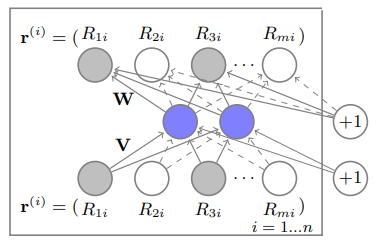
\includegraphics[keepaspectratio]{figures/algorithms/auto_rc.PNG}
    \caption{Modello AutoRec basato sugli \textit{item}. Si utilizza la notazione a piatto per indicare che ci sono $n$ copie della rete neurale (una per ciascun \textit{item}), dove $W$ e $V$ sono condivisi tra tutte le copie.}
    \label{fig:auto_rec}
\end{figure}

Un tipico autoencoder è composto da un \textit{encoder} e un \textit{decodificatore}. L'\textit{encoder} proietta l'input verso rappresentazioni nascoste e il \textit{decodificatore} mappa il livello nascosto al livello di ricostruzione. Nessuna funzione di attivazione è applicata al \textit{decodificatore}. Il \textit{dropout} è incluso dopo l'\textit{encoding} per ridurre l'overfitting. I gradienti degli input non osservati vengono mascherati per garantire che solo le valutazioni osservate contribuiscano al processo di apprendimento del modello.

Per l'addestramento si può utilizzare \textit{L2 loss} e come metrica di accuratezza l'\textit{RMSE}.

\begin{itemize}
  \item semplice da implementare: la struttura autoencoder consente una modellazione diretta delle preferenze degli \textit{user} o degli \textit{item}
  \item compatto: il modello ha pochi parametri e richiede meno risorse computazionali rispetto a modelli più complessi
  \item efficace per dati sparsi: grazie alla ricostruzione degli input, riesce a gestire bene la mancanza di interazioni esplicite
\end{itemize}

L'algoritmo soffre anche di diverse problematiche:

\begin{itemize}
  \item limitato nella modellazione delle interazioni complesse: non riesce a catturare relazioni non lineari sofisticate tra \textit{user} e \textit{item}
  \item feeedback espliciti: il modello utilizza i feedback espliciti per l'addestramento, più difficili da reperire
  \item richiede due versioni distinte per \textit{user-based} e \textit{item-based}: non esiste una versione unificata che modelli entrambi simultaneamente
\end{itemize}

\subsection{NCF}\label{ncf}
Viene introdotto il framework di \textit{Neural Collaborative Filtering} (\textit{NCF}) per sistemi di raccomandazione basati su feedback implicito.

Il modello, chiamato \textit{Neural Matrix Factorization} (\textit{NeuMF})~\cite{NeuMF} mira ad affrontare il compito di ordinamento personalizzato basato su feedback implicito. Questo modello sfrutta la flessibilità e la non-linearità delle reti neurali per sostituire i prodotti scalari della fattorizzazione di matrici, con l'obiettivo di aumentare l'espressività del modello.

In particolare, il modello è composto da due sottoreti: \textit'{Generalized Matrix Factorization} (\textit{GMF}) e una rete \textit{Multi-Layer Perceptron} (\textit{MLP}), e modella le interazioni attraverso due percorsi distinti anziché usare un semplice prodotto scalare. Gli output di queste due reti sono concatenate per calcolare il punteggio finale di predizione.

Diversamente dal compito di previsione dei \textit{rating} (come in \textit{AutoRec}~\ref{autorec}), questo modello genera una lista ordinata di raccomandazioni per ciascun \textit{user} basata su feedback implicito.

\subsubsection{Il modello NeuMF}\label{neufm}

\textit{NeuMF} fonde due sottoreti. La \textit{GMF} è una versione neurale generica della fattorizzazione di matrici, in cui l'input è il prodotto elemento per elemento (\textit{Hadamard}) dei fattori latenti dello \textit{user} e dell'\textit{item}. Essa consiste in due layer neurali:

\[
\begin{split}
x &= p_u \odot q_i \\
\hat{y}_{ui} &= \alpha(h^\top x),
\end{split}
\]

dove $\odot$ rappresenta l'\textit{Hadamard product} tra vettori, $P \in \mathbb{R}^{m \times k}$ e $Q \in \mathbb{R}^{n \times k}$ sono rispettivamente la matrice latente degli utenti e quella degli oggetti, $p_u \in \mathbb{R}^{k}$ è la riga $u$-esima di $P$, $q_i \in \mathbb{R}^{ k}$ è la riga $i$-esima di $Q$, $a$ è la funzione di attivazione, e $h$ è il vettore dei pesi dell'output layer.  
$\hat{y}_{ui}$ è il punteggio predetto che lo \textit{user} $u$ potrebbe assegnare all'\textit{item} $i$.

L'altro componente del modello è la \textit{MLP}. Per aumentare la flessibilità del modello, le embedding di \textit{user} e \textit{item} non sono condivise con la \textit{GMF}. Il \textit{MLP} utilizza la concatenazione delle embedding come input. Grazie a connessioni complesse e trasformazioni non lineari, è in grado di modellare interazioni sofisticate tra utenti e oggetti. Più precisamente:

\[
\begin{aligned}
z^{(1)} &= \phi_1(U_u, V_i) = \left[ U_u, V_i \right] \\
\phi^{(2)}(z^{(1)}) &= \alpha^1(W^{(2)} z^{(1)} + b^{(2)}) \\
&\dots \\
\phi^{(L)}(z^{(L-1)}) &= \alpha^L(W^{(L)} z^{(L-1)} + b^{(L)}) \\
\hat{y}_{ui} &= \alpha(h^\top \phi^L(z^{(L-1)}))
\end{aligned}
\]


dove $W^*$, $b^*$ e $\alpha^*$ sono rispettivamente la matrice dei pesi, il vettore di bias e la funzione di attivazione. $\phi^*$ denota la funzione del layer corrispondente mentre $z^*$ è l'output del layer corrispondente.

Per combinare i risultati di \textit{GMF} e \textit{MLP}, invece della semplice somma, \textit{NeuMF} concatena i penultimi layer delle due sottoreti per creare un vettore di features che viene passato a un ulteriore layer. Successivamente, gli output vengono proiettate con la matrice $h$ e una funzione di attivazione sigmoide. L'output finale è calcolato come:

\[
\hat{y}_{ui} = \sigma(h^\top[x, \phi^L(z^{(L-1)})]).
\]

\begin{figure}[H]
    \centering
    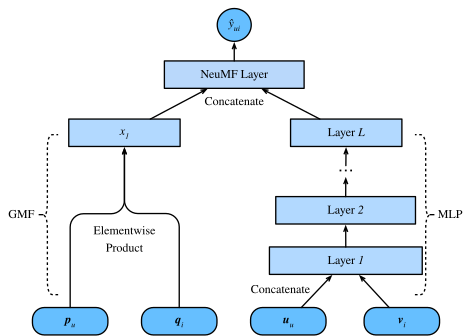
\includegraphics[scale=0.6]{figures/algorithms/neu_mf.png}
    \caption{Modello \textit{NeuMF}}
    \label{fig:neu_mf}
\end{figure}

\textit{NeuMF} consiste in un modello di \textit{Generalized Matrix Factorization} (\textit{GMF}) e una rete neurale \textit{Multi-Layer Perceptron} (\textit{MLP}) con vettori di \textit{embedding} distinti per utenti e \textit{item}. La struttura dell'MLP è controllata dal parametro \\ \texttt{nums\_hiddens}. \textit{ReLU} è utilizzata come funzione di attivazione predefinita.

Come \textit{loss} si utilizza la \textit{binary cross entropy}, conosciuta anche come \textit{log loss}, in cui un passaggio importante è il campionamento negativo. 
\[
\mathcal{L} = -\sum_{(u,i) \in Y \cup Y^{-}} \left[ y_{ui} \cdot \log \hat{y}_{ui} + (1 - y_{ui}) \cdot \log(1 - \hat{y}_{ui}) \right]
\]

Per ogni \textit{user}, gli \textit{item} con cui lo \textit{user} non ha interagito sono considerati \textit{item} candidati (voci non osservate). Durante la fase di addestramento, il modello si assicura che gli \textit{item} che uno \textit{user} gradisce vengano classificati più in alto rispetto agli \textit{item} che lo \textit{user} non gradisce o con cui non ha interagito.

I punti di forza dell'algoritmo sono:

\begin{itemize}
  \item maggiore capacità espressiva: rispetto ad \textit{AutoRec} usa reti neurali profonde per modellare interazioni non lineari tra \textit{user} e \textit{item}
  \item flessibile: consente l'integrazione di moduli diversi (\textit{GMF}, \textit{MLP}) in un'unica architettura
  \item end-to-end: apprende le rappresentazioni e le interazioni simultaneamente durante l'addestramento
\end{itemize}

L'algoritmo soffre anche di diverse problematiche:

\begin{itemize}
  \item più costoso computazionalmente: richiede più memoria e potenza di calcolo rispetto ad \textit{AutoRec}
  \item può soffrire di overfitting: l'alta capacità del modello può portare a una scarsa generalizzazione sui dati di test
  \item necessita di tuning accurato: le prestazioni dipendono fortemente dall'architettura e dagli iperparametri
\end{itemize}

\subsection{DeepFM}

Le reti neurali profonde sono potenti nell’apprendimento della rappresentazione delle caratteristiche e hanno il potenziale per apprendere interazioni sofisticate. Grazie a livelli di trasformazione non lineare si ottiene la capacità di modellare sia combinazioni di caratteristiche di basso ordine sia di alto ordine. Inoltre, le strutture intrinsecamente non lineari degli input possono essere catturate dalle reti neurali profonde. 

Si introduce un modello rappresentativo chiamato \textit{Deep Factorization Machines} (\textit{DeepFM})~\cite{DeepFM}.

\textit{DeepFM} è composto da una componente di \textit{Factorization Machine} (\textit{FM}) e da una componente deep, integrate in una struttura parallela. La componente \textit{FM} è identica alla \textit{2-Way Factorization Machine}, utilizzata per modellare le interazioni tra caratteristiche di basso ordine. La componente deep è una rete \textit{Multi Layer Perceptron} (MLP), usata per catturare interazioni tra caratteristiche di ordine superiore e non linearità.

Queste due componenti condividono gli stessi input/\textit{embedding}, e i loro output vengono sommati per ottenere la previsione finale.

\subsubsection{2-Way Factorization Machine}

Le \textit{Factorization Machines} (\textit{FM}), proposte da \textit{Rendle}~\cite{FM}, sono algoritmi supervisionati che possono essere utilizzati per attività di classificazione, regressione e ranking. Hanno rapidamente preso piede e sono diventati un metodo popolare e di impatto per fare previsioni e raccomandazioni. In particolare, rappresentano una generalizzazione del modello di regressione lineare e del modello di fattorizzazione di matrici. Inoltre, ricordano le macchine a vettori di supporto con un kernel polinomiale. I punti di forza delle \textit{Factorization Machines} rispetto alla regressione lineare e alla fattorizzazione di matrici sono: 
\begin{itemize}
    \item possono modellare interazioni variabili a $\chi$ vie, dove $\chi$ è il numero di ordine polinomiale ed è solitamente impostato a due
    \item un algoritmo di ottimizzazione veloce associato alle \textit{Factorization Machines} può ridurre il tempo di calcolo del polinomio a una complessità lineare, rendendolo estremamente efficiente soprattutto per input sparsi di elevata dimensionalità
\end{itemize}

Per questi motivi, le \textit{Factorization Machines} sono ampiamente utilizzate nella pubblicità moderna e nelle raccomandazioni di prodotto.


Formalmente, sia $x \in \mathbb{R}^d$ il vettore delle caratteristiche di un campione, e $y$ l'etichetta corrispondente, che può essere un valore reale o un'etichetta di classe, come ad esempio una classe binaria "click/non-click".  
Il modello per una factorization machine di grado due è definito come:

\[
\hat{y}(x) = \mathbf{w}_0 + \sum_{i=1}^d \mathbf{w}_i x_i + \sum_{i=1}^d\sum_{j=i+1}^d \langle\mathbf{v}_i, \mathbf{v}_j\rangle x_i x_j
\]

dove $w_0 \in \mathbb{R}$ è il bias globale; $w \in \mathbb{R}^d$ denota i pesi della i-esima variabile; $V \in \mathbb{R}^{d\times k}$ rappresenta le embedding delle feature; $v_i$ rappresenta l'$i$-esima riga di $V$; $k$ è la dimensionalità dei fattori latenti; $\langle\cdot, \cdot \rangle$ è il prodotto scalare di due vettori.

$\langle \mathbf{v}_i, \mathbf{v}_j \rangle$ rappresenta l'interazione tra la $i$-esima e la $j$-esima feature. Alcune interazioni tra feature possono essere facilmente comprese, quindi possono essere progettate dagli esperti. Tuttavia, la maggior parte delle altre interazioni tra feature sono nascoste nei dati e difficili da identificare. Pertanto, modellare automaticamente le interazioni tra feature può ridurre notevolmente gli sforzi nell'ingegneria delle feature. È evidente che i primi due termini corrispondono al modello di regressione lineare e l'ultimo termine è un'estensione del modello di fattorizzazione della matrice. Se la feature $i$ rappresenta un articolo e la feature $j$ rappresenta un utente, il terzo termine è esattamente il prodotto scalare tra le embedding dell'utente e dell'articolo.

Da notare che il modello \textit{FM} può anche generalizzarsi a ordini superiori (grado > 2). Tuttavia, la stabilità numerica potrebbe indebolire la generalizzazione.

Ottimizzare le \textit{FM} in un modo diretto porta a una complessità di $\mathcal{O}(kd^2)$ poiché tutte le interazioni a coppie devono essere calcolate. Per risolvere questo problema di inefficienza, si può riorganizzare il terzo termine di \textit{FM}, il che potrebbe ridurre notevolmente il costo computazionale, portando a una complessità temporale lineare $\mathcal{O}(kd)$. La riformulazione del termine di interazione a coppie è la seguente:

\[
\begin{split}\begin{aligned}
&\sum_{i=1}^d \sum_{j=i+1}^d \langle\mathbf{v}_i, \mathbf{v}_j\rangle x_i x_j \\
 &= \frac{1}{2} \sum_{i=1}^d \sum_{j=1}^d\langle\mathbf{v}_i, \mathbf{v}_j\rangle x_i x_j - \frac{1}{2}\sum_{i=1}^d \langle\mathbf{v}_i, \mathbf{v}_i\rangle x_i x_i \\
 &= \frac{1}{2} \big (\sum_{i=1}^d \sum_{j=1}^d \sum_{l=1}^k\mathbf{v}_{i, l} \mathbf{v}_{j, l} x_i x_j - \sum_{i=1}^d \sum_{l=1}^k \mathbf{v}_{i, l} \mathbf{v}_{i, l} x_i x_i \big)\\
 &=  \frac{1}{2} \sum_{l=1}^k \big ((\sum_{i=1}^d \mathbf{v}_{i, l} x_i) (\sum_{j=1}^d \mathbf{v}_{j, l}x_j) - \sum_{i=1}^d \mathbf{v}_{i, l}^2 x_i^2 \big ) \\
 &= \frac{1}{2} \sum_{l=1}^k \big ((\sum_{i=1}^d \mathbf{v}_{i, l} x_i)^2 - \sum_{i=1}^d \mathbf{v}_{i, l}^2 x_i^2)
 \end{aligned}\end{split}
\]

Con questa riformulazione, la complessità del modello diminuisce notevolmente. Inoltre, per le feature sparse, è necessario calcolare solo gli elementi non nulli, in modo che la complessità complessiva sia lineare rispetto al numero di feature non nulle.
La predizione finale diventa:

\[
\hat{y}(x) = w_0 + \sum_{i=1}^d w_i x_i + \frac{1}{2} \sum_{l=1}^k \left( \left( \sum_{i=1}^d v_{i,l} x_i \right)^2 - \sum_{i=1}^d v_{i,l}^2 x_i^2 \right)
\]

\subsubsection{Architettura DeepFM}
Si denota l'output della componente \textit{FM} come $\hat{y}^{(FM)}$. Sia $e_i \in \mathbb{R}^{k}$ il vettore di caratteristiche latenti (\textit{embedding}) dell'$i$-esimo campo. L'input della componente deep è la concatenazione degli \textit{embedding} densi di tutti i campi, ottenuti a partire dalle caratteristiche categoriali sparse in input, ed è denotato come:

\[
\mathbf{z}^{(0)} = [\mathbf{e}_1, \mathbf{e}_2, \ldots, \mathbf{e}_f]
\]

dove $f$ è il numero totale di campi. Viene quindi passato alla rete neurale seguente:
\[
\mathbf{z}^{(l)}  = \alpha(W^{(l)}z^{(l-1)} + b^{(l)}),
\]

dove $\alpha$ è la funzione di attivazione. $W_l$ e $b_l$ sono rispettivamente pesi e bias dell'$l^{th}$ layer. I parametri della rete includono pesi e bias specifici per ciascun livello. Sia $y_{DNN}$ l'output della parte \textit{MLP}. Il risultato finale è ottenuto sommando i risultati prodotti sia dalla componente \textit{FM} che dalla rete neurale profonda (\textit{DNN}). Questa somma viene infine elaborata dalla funzione sigmoide per produrre la probabilità finale:

\[
\hat{y} = \sigma(\hat{y}^{(FM)} + \hat{y}^{(DNN)})
\]

dove $\sigma$ è la funzione sigmoide.

\begin{figure}[H]
    \centering
    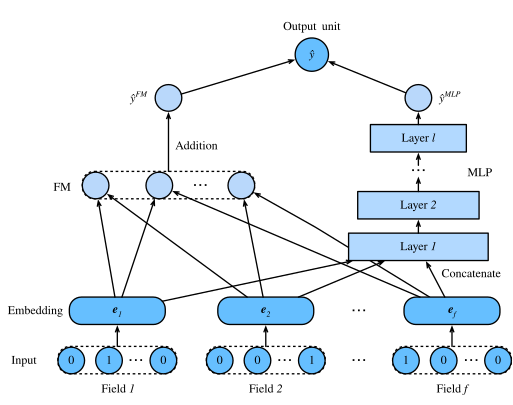
\includegraphics[scale=0.5]{figures/algorithms/deepfm.png}
    \caption{L'architettura di \textit{DeepFM}. In questa immagine $\hat{y}^{(MLP)} = \hat{y}^{(DNN)}$}
    \label{fig:deepfm}
\end{figure}

Importante sottolineare che \textit{DeepFM} non è l'unico modo per combinare reti neurali profonde con \textit{FM}. Si possono aggiungere livelli non lineari sulle interazioni tra le caratteristiche~\cite{NFA_SPA}.

Come per \textit{NeuMF}~\ref{neufm} la \textit{loss} utilizzata è la \textit{binary cross entropy}.

I punti di forza dell'algoritmo sono:

\begin{itemize}
  \item estende \textit{NCF} con la componente delle \textit{Factorization Machine}: migliora la modellazione delle interazioni bilineari esplicite tra caratteristiche
  \item sfrutta sia caratteristiche sparse che dense: efficace anche su dati con numerosi campi categoriali
  \item end-to-end senza feature engineering: apprende automaticamente le interazioni complesse tra caratteristiche
\end{itemize}

L'algoritmo soffre anche di diverse problematiche:

\begin{itemize}
  \item maggiore complessità rispetto a \textit{NCF}: la combinazione di \textit{FM} e \textit{MLP} rende il modello più difficile da addestrare
  \item richiede una gestione attenta delle feature: la qualità delle embedding iniziali può influenzare fortemente le performance
  \item può essere meno interpretabile: l'uso congiunto di \textit{FM} e deep learning rende l'analisi dei risultati più opaca
\end{itemize}

\section{Evaluation}\label{evaluation}

In un sistema di \textit{recommendation}, è fondamentale misurare l'efficacia delle raccomandazioni prodotte in base all'interazione dell'utente con gli \textit{item} proposti. Prima di poter elencare alcune delle metriche più utilizzate occorre specificare la notazione utilizzata:

\begin{itemize}
    \item $I_u^{rel}$ è l'insieme degli \textit{item} rilevanti per $u$, ovvero quelli per cui $r_{ui}$ è maggiore o uguale a una certa soglia di rilevanza (es. $4$ su una scala $1-5$) nel caso di feedback espliciti. Nel caso di feedback impliciti, $I_u^{rel}$ è l'insieme degli \textit{item} con cui l'utente ha \textit{interagito} (es. clic, acquisti, visualizzazioni, ascolti, ecc.). In un contesto di feedback implicito, l'interazione è sufficiente per considerare un \textit{item} come rilevante, senza la necessità di una soglia numerica.
    \item $\hat{I}_u^K$ è l'insieme dei \textit{top-K item} raccomandati allo \textit{user} $u$, ottenuto ordinando in modo decrescente gli \textit{item} in $I \setminus I_u$ in base allo \textit{rating} $\hat{r}_{ui}$ o \textit{score} $\hat{y}_{ui}$, rispettivamente per feedback espliciti e impliciti, e prendendo i primi $K$.
    \item L'insieme degli \textit{item} rilevanti tra i top-K per $u$ è dato da:
    \[
    I_u^{rel@K} = \hat{I}_u^K \cap I_u^{rel}
    \]
    che rappresenta il numero di \textit{item} che appaiono tra i top-K raccomandati e con cui l'utente ha già interagito o che risultano rilevanti a seconda che si tratti di feedback espliciti o impliciti.
    \item L'insieme degli \textit{item} non rilevanti, ovvero quelli con cui l'utente non ha mai interagito, è dato da:
    \[
    I_u^{non-rel} = I \setminus I_u^{rel}
    \]
    che corrisponde agli \textit{item} mai interagiti dall'utente. Nel contesto dei feedback impliciti, questi \textit{item} potrebbero essere semplicemente quelli non ancora scoperti dall'utente, quindi la loro rilevanza non è assolutamente garantita.
\end{itemize}




Di seguito sono presentate le definizioni formali di ciascuna di queste metriche.

Le prime due metriche hanno senso solamente per feedback espliciti in quanto restituiscono un \textit{rating}:

\begin{itemize}
    \item Root Mean Squared Error (RMSE).\\
    Errore quadratico medio tra i punteggi previsti e quelli reali; penalizza di più gli errori grandi.
    \[
    \text{RMSE} = \sqrt{ \frac{1}{|\hat{R}|} \sum_{\hat{r}_{ui} \in \hat{R}} (\hat{r}_{ui} - r_{ui})^2 }
    \]
    
    \item Mean Absolute Error (MAE).\\
    Errore assoluto medio tra le predizioni e i valori reali; più facile da interpretare rispetto a RMSE.
    \[
    \text{MAE} = \frac{1}{|\hat{R}|} \sum_{\hat{r}_{ui} \in \hat{R}} |\hat{r}_{ui} - r_{ui}|
    \]
\end{itemize}   

Le seguenti metriche valgono sia per feedback impliciti che espliciti:

\begin{itemize}
    \item Precision@K.\\
    Frazione dei top-K \textit{item} raccomandati che sono effettivamente rilevanti.
    \[
    \text{Precision@K}(u) = \frac{|I_u^{rel@K}|}{K}
    \]
    
    \item Recall@K.\\
    Frazione degli \textit{item} rilevanti che sono stati inclusi nei top-K raccomandati.
    \[
    \text{Recall@K}(u) = \frac{|I_u^{rel@K}|}{|I_u^{rel}|}
    \]
    
    \item F1@K.\\
    Media armonica tra precision@K e recall@K; è alta solo se entrambe le metriche sono alte.
    \[
    \text{F1@K}(u) = 2 \cdot \frac{\text{Precision@K}(u) \cdot \text{Recall@K}(u)}{\text{Precision@K}(u) + \text{Recall@K}(u)}
    \]
    \item Hit@K.\\
    Metrica binaria che indica se almeno un \textit{item} rilevante per lo \textit{user} compare tra i primi K raccomandati. Se sì, il valore è 1 (hit), altrimenti 0 (miss). Misura la capacità del sistema di \textit{recommendation} di "azzeccare" almeno una preferenza dello \textit{user} nelle top-K proposte.\\
    \[
    \text{oppure} \quad 
    \text{Hit@K}(u) = \mathbf{1}\left\{ |I_u^{rel@K}| > 0 \right\}
    \]  
    
    \item Area Under the ROC Curve (AUC).\\
    Probabilità che un \textit{item} rilevante riceva uno \textit{score} più alto rispetto a un \textit{item} non rilevante.
    \[
    \text{AUC}(u) = \frac{1}{|I_u^{rel}| \cdot |I_u^{non-rel}|} \sum_{i \in I_u^{rel}} \sum_{j \in I_u^{non-rel}} \mathbf{1}\{\hat{r}_{ui} > \hat{r}_{uj}\}
    \]
    
    \item Normalized Discounted Cumulative Gain (NDCG@K).\\
    Premia le raccomandazioni rilevanti che si trovano in alto nella lista, simulando la probabilità che vengano viste.
    \[
    \text{DCG@K}(u) = \sum_{k=1}^{K} \frac{\mathbf{1}\{i_k \in I_u^{rel}\}}{\log_2(k + 1)}
    \]
    \[
    \text{IDCG@K}(u) = \sum_{k=1}^{\min(K, |I_u^{rel}|)} \frac{1}{\log_2(k + 1)}
    \]
    \[
    \text{NDCG@K}(u) = \frac{\text{DCG@K}(u)}{\text{IDCG@K}(u)}
    \]
\end{itemize}